\documentclass[TS]{sesamanuel}

% modifications dans la classe (fichier sesamanuel.cls) :
% 	1) ligne 2873, la ligne de remise à zéro du compteur de chapitre a été commentée pour "themaG"
% 	2) création d'une boîte à connaître à la ligne 3471
%	3) ligne 2141 : définition de trois couleurs utilisé par les anciennes figures libreoffice
%	4) ligne 179 et 180 ajout de 2 lignes pour utiliser la police pazocal qui modifie les caractères calligraphiés en mode math
%		du coup : \mathcal{C} donne un C fortement calligraphié et \pazocal{C} donne l'habituel C calligraphié de mathcal
%	5) suppression du texte et du logo dans le titre des QCM d'autoévaluation "Ressources dispo sur sesamaths..." :
%		lignes 3117 et 4396 : commande \StringManuel est commentée
%		lignes 3122 et 4401 : je n'ai pas supprimé le \LogoManuel (une @) mais j'ai changé sa couleur de U4 à Blanc (à la ligne 2702)

% modifications dans le fichier commandesTikZ :
% lignes 31 et 32 pour ajouter la commande \circled qui entoure un caractère



%%%%%%%
%Rajouté le 12/06/2018 SV et BN pour compilation espace insécable sous linux 
\DeclareUnicodeCharacter{00A0}{~} %pour remplacer les espaces insécables
\DeclareUnicodeCharacter{2011}{-}
%\usepackage{pdfpages}
%%%%%%%

\input{commandes-manuel-TS} % pour l'instant on garde sinon les corrigés ne sont
						% pas dans classés dans un dossier "correction"
\input{commandes-tikz}

\graphicspath{%
  {ex1/figures/}%
  {LesRacinesCarrees/figures/}%
  {LesTheoremes/figures/}%
  {Degre1/figures/}%
  {Images/}%
}


% création d'un nouveau thème "calcul" pour le document
\NewThema{C}{c}{calcul}{Calcul}{}{PartieFonction}{A3}

\renewcommand\ListeMethodesThemes{{c}{C},{g}{G}}
\renewcommand*\StringListeMethode{M\'ethodes du livret 1}

% création d'un nouveau thème "Manuel" pour le sommaire
\NewThema{M}{m}{manuel}{Manuel}{MANUEL}{PartieFonction}{A3}

\begin{document}

%%%%%%%%%%%%%%%%%%%%%%
%Couverture inclusion page entière en eps
\pagestyle{empty}

\includegraphics[width=.92\textwidth]{couverture}

\newpage \pagestyle{empty}
\addto\captionsfrench{\renewcommand{\contentsname}{Sommaire}}

%\setcounter{tocdepth}{2}


%%%%%%%%%%%%%%%%%%%%%%%%%%
% Table des matières
%%%%%%%%%%%%%%%%%%%%%%%%%%

\themaM %thème déclaré en début de document
\colorlet{ChapterNumColor}{PartieFonction}
\chapter{Manuel de Troisième\\Maturité Standard}

\vfill

\begin{commentaire}

\textcolor{PartieFonction}{\PrerequisTitleFont 
Chapitre \ref{ChCalAlgebriques}: Calculs algébriques \dotfill\ page \pageref{ChCalAlgebriques}}

\vspace{2em}

\textcolor{PartieGeometrie}{\PrerequisTitleFont 
Chapitre \ref{ChLesVecteurs}: Les vecteurs 1 \dotfill\ page \pageref{ChLesVecteurs}}

\vspace{2em}

\textcolor{PartieFonction}{\PrerequisTitleFont 
Chapitre \ref{ChLesRacinesCarrees}: Les Racines Carrées \dotfill\ page \pageref{ChLesRacinesCarrees}}

\vspace{2em}

\textcolor{PartieGeometrie}{\PrerequisTitleFont 
Chapitre \ref{ChLesTheoremes}: Les théorèmes en géométrie \dotfill\ page \pageref{ChLesTheoremes}}

\vspace{2em}

\textcolor{PartieFonction}{\PrerequisTitleFont 
Chapitre \ref{ChDegre1}: Equations et inéquations de degré 1 \dotfill\ page \pageref{ChDegre1}}

\vspace{2em}

\textcolor{PartieFonction}{\PrerequisTitleFont 
Chapitre \ref{ChPerimetresAires}: Nombres entiers et décimaux \dotfill\ page \pageref{ChPerimetresAires}}

\vspace{2em}

\end{commentaire}

\vfill

%%%%%%%%%%%%%%%%%%%%%%%%%%
% Fin table des matières
%%%%%%%%%%%%%%%%%%%%%%%%%%

%%%%%%%%%%%%%%%%%%%%%%%%%%
%Page Sesamath
%%%%%%%%%%%%%%%%%%%%%%%%%%
\newpage


\begin{prerequis}[Un manuel de l'association Sésamath]
\begin{itemize}
\item  Ce manuel est adapté en partie du manuel Sésamath de l'association Sésamath:\\
\texttt{http://manuel.sesamath.net/}
\item … Et de l'association Sésamath Suisse romande:\\ \texttt{http://www.sesamath.ch/}
\item L'Institut Florimont a réalisé la transcription dans le langage de description de documents libre et gratuit \LaTeX{} en utilisant la classe \texttt{sesamanuel} développée par l'association Sésamath;
\item E. Villié a réalisé la couverture pour l'Institut Florimont;
\item Version juin 2018 --- Institut Florimont (Genève).
\end{itemize}
 \end{prerequis}

\vspace{10em}




%%%%%%%%%%%%%%%%%%%%%%%%%%
%Fin page Sesamath
%%%%%%%%%%%%%%%%%%%%%%%%%%

\colorlet{ChapterNumColor}{white}
\setcounter{chapter}{0}

%\themaC
%\themaG


\setcounter{page}{6}

\themaC
\chapter{Calculs Algébriques}\label{ChCalAlgebriques}



%\activites

%\input{NombresEntiersDecimaux/NbEntDec_acti.tex}

\begin{acquis}
\begin{itemize}
\item Savoir calculer avec les puissances;
\item Savoir utiliser l'écriture scientifique;
\item Savoir développer une expression;\\
\item Savoir factoriser une expression en cherchant un facteur commun;
\item Savoir factoriser une expression en utilisant les identités remarquables.
\end{itemize}
\end{acquis}

%\cours
%\begin{acquis}
\begin{itemize}
\item Savoir calculer avec les puissances;
\item Savoir utiliser l'écriture scientifique;
\item Savoir développer une expression;
\item Savoir factoriser une expression en cherchant un facteur commun;
\item Savoir factoriser une expression en utilisant les identités remarquables.
\end{itemize}
\end{acquis}





\exercicesbase
\begin{colonne*exercice}
 \definecolor{fondTI}{HTML}{869286}


\serie{Puissances}

\begin{exercice}[]
Ecrire chaque expression sous la forme d'une fraction irréductible.\\

\begin{tabular}{p{1,1cm}p{0,8cm}p{1cm}p{0,8cm}p{1cm}p{0,8cm}}
$7^{-2}=$ & & \scriptsize $(-6)^{-1}=$ & & $4^{-3}=$ & \\
& ....... & & ....... & & .......\\
\end{tabular}
\end{exercice}
\medskip
\begin{exercice}[]
Calculer mentalement et exprimer sous la forme d'une fraction lorsque le résultat n'est pas un nombre entier.

\renewcommand{\arraystretch}{1.1}
\begin{tabular}{p{1,1cm}p{0,8cm}p{1cm}p{0,8cm}p{1cm}p{0,8cm}}
$(-5)^2 =$ & ....... & $5^{-2} =$ & ....... & $-5^2 =$ & .......\\
&&&&&\\
$5^3 =$ & ....... & $(-5)^3=$ & ....... & $1^6=$ & .......\\
&&&&&\\
$(-3)^4 =$ & ....... & \scriptsize $-(-4)^2 =$ & ....... & \scriptsize $2014^0 =$ & .......\\
&&&&&\\
$-2^3 =$ & ....... & $(-2)^3 =$ & ....... & $2^{-1} =$ & .......\\
&&&&&\\
\scriptsize $(-2)^{-1} =$ & ....... & $3^{-2} =$ & ....... & \scriptsize $2015^1 =$ & .......\\

\end{tabular}
\end{exercice}
\medskip
\begin{exercice}[]
Compléter chaque égalité à l'aide d'un exposant entier relatif.

\begin{tabular}{p{2cm}p{2,75cm}p{2,5cm}}
$25 = 5^{.....}$ & $-27 = (-3)^{.....}$ & $49 = 7^{.....}$\\
&&\\
$\dfrac{1}{4} = 2^{.....}$ & $\dfrac{5}{7} = \left(\dfrac{7}{5}\right)^{.....}$& $\dfrac{27}{8} = \left(\dfrac{3}{2}\right)^{.....}$\\
\end{tabular}
\end{exercice}
\medskip
\begin{exercice}[]
Ecrire chaque nombre sous la forme $a^n$,

où $a$ et $n$ sont des nombres entiers relatifs.

(a) 32 \hspace{0.5cm} (b) 27 \hspace{0.5cm} (c) 100 000 \hspace{0.5cm} (d) $\dfrac{1}{81}$
\end{exercice}
\medskip
\begin{exercice}[]
Calculer chaque expression en détaillant les étapes.

\begin{tabular}{m{3.8cm}m{3.5cm}}
A = $2 + 2^3 \times 5^2$ & B = $-3^2 + 8 : 2^2$\\
&\\
C = $2^2 + 2^{-2}$ & D = $2^2 \times 2^{-2}$\\
&
\end{tabular}
\end{exercice}
\medskip
\begin{exercice}[]
Ecrire chaque expression sous la forme $a^n$,

où $n$ est un nombre entier relatif.

\renewcommand{\arraystretch}{0.8}
\begin{tabular}{p{4cm}p{4cm}}
(a) $3^2 \times 3^5$ & (b) $(-6)^{10} \times (-6)^7$\\
&\\
(c) $\left(\dfrac{5}{3}\right)^4 \times \left(\dfrac{5}{3}\right)^3$ & (d) $\left(\dfrac{4}{7}\right)^8 \times \dfrac{4}{7}$\\
&\\

(e) $\left(\dfrac{1}{3}\right)^{12} \times \left(\dfrac{1}{3}\right)^{-7}$ & (f) $(-9)^{-8} \times (-9)$\\
&\\
(g) $\dfrac{2^6}{2^4}$ & (h) $\dfrac{5^{-3}}{5^7}$\\
&\\

(i) $\left(2^3\right)^4$ & (j) $\left(1,2^5\right)^{-2}$\\
&\\
(k) $\left(\left(\dfrac{5}{6}\right)^{-1}\right)^4$ & (l) $\left(\left(-2\right)^{-6}\right)^{-7}$\\
&\\
(m) $9^2 \times 7^2$ & (n) $(-11)^{-1} \times 3^{-1}$\\
&\\
(o) $(-5)^{-6} \times (-7)^{-6}$ & (p) $\left(\dfrac{2}{3}\right)^5 \times \left(\dfrac{9}{10}\right)^5$\\
&\\
(q) $\dfrac{24^7}{3^7}$ & (r) $\dfrac{(-4,5)^{-3}}{9^{-3}}$\\
\end{tabular}
\end{exercice}
\medskip
\begin{exercice}[]
Pour chacune des écritures suivantes :
\begin{itemize}
\item dire s'il s'agit ou non d'une écriture scientifique ;
\item donner son écriture décimale.
\end{itemize}

\renewcommand{\arraystretch}{0.8}
\begin{tabular}{p{4cm}p{4cm}}
(a) $5 \times 10^4$ & (b) $21,8 \times 10^6$\\
&\\
(c) $6,5 \times 10^{-2}$ & (d) $0,4 \times 10^{-5}$\\
&\\
(e) $-3 000 \times 10^{-6}$ & (f) $-1,7 \times 10^{-1}$\\
\end{tabular}
\end{exercice}
\medskip
\begin{exercice}[]
Donner l'écriture scientifique de chacun des nombres suivants.

\renewcommand{\arraystretch}{0.8}
\begin{tabular}{p{4cm}p{4cm}}
(a) $471$ & (b) $-360~000$\\
&\\
(c) $0,025$ & (d) $1234,567$\\
&\\
(e) $920~000~000$ & (f) $-0,000~000~000~03$\\
\end{tabular}
\end{exercice}
\medskip
\begin{exercice}[]
Calculer les expressions suivantes et donner l'écriture scientique du résultat.
\begin{description}
\item $A=\dfrac{90 \times 10^7 \times 1,4 \times10^{-2}}{12 \times (10^3)^5}$\\
\item $B=\dfrac{2400 \times 10^{-3} \times 0,28 \times10^{-2}}{8,4 \times (10^{-10})^2}$
\end{description}
\end{exercice}

\newpage

\serie{Développer et factoriser}

\begin{exercice}[]
Développer et réduire les expressions algébriques suivantes :

\begin{tabular}{m{4.75cm}m{2.75cm}}
{A$_1=8 \times (-6x-9)+1$} \\
&\\
{A$_2=6x+5 \times (-5x-2)$}\\
&\\
{A$_3=10 \times (x-4)+4x+3$}\\
\end{tabular}
\end{exercice}

\begin{exercice}[]
Développer et réduire les produits suivants :

\begin{tabular}{m{5.75cm}m{1.75cm}}
B$_1=(x+2) \times (x+5)$ \\
&\\
B_2 {$=\left(x+\dfrac{5}{4} \right) \left (3x-\dfrac{1}{2} \right)$}
&\\
B$_3=(2x-3)x+(x+5)(3x-4)$\\
&\\
B$_4=(6-a)(2a+5)-(-a+1)(3a-10)$}\\
\end{tabular}
\end{exercice}

\begin{exercice}[]
Factoriser chacune des expressions suivantes, en identifiant au préalable un facteur commun :

\footnotesize \hspace{0.5cm}
\begin{tabular}{m{3.75cm}m{3.75cm}}
C$_1=3x-9$ & C$_2=6,3y+6,3$\\
&\\
C$_3=5x-12x^2$ & C$_4=60a^2-120a$\\
&\\
C$_5=b^4+3b^2$ & C$_6=48x^3+16x^2-32x$\\\\
\end{tabular}
\end{exercice}

\begin{exercice}[]
Développer et réduire les produits suivants, en utilisant une des trois premières identités remarquables :

\vspace{0.25cm}
\begin{tabular}{m{3.75cm}m{3.75cm}}
D$_1=(x+2)^2$ & D$_2=(a-5)^2$\\
&\\
D$_3=\left(x+\dfrac{2}{3} \right)^2$ & D$_4=(7-5x)(7+5x)$\D$_1=(x+2)^2$ & D$_2=(a-5)^2$\\
&\\
D$_5=\left(5x-10 \right)^2$ & D$_6=(5x-10)(5x+10)$\\
&\\
D$_7=(5x-2)^2$ & D$_8=(3x-4)(4+3x)$\\
&\\
D$_9=\left(\dfrac{4}{7}x- \dfrac{4}{3} \right)^2$ & D$_10=-(9x-5)(5-9x)$\\
\end{tabular}
\end{exercice}

\begin{exercice}[]
Factoriser, lorsque c'est possible, chacune des expressions suivantes, en utilisant une des trois premières identités remarquables :

\vspace{0.25cm}
\begin{tabular}{m{3.75cm}m{3.75cm}}
E$_1=x^2+6x+9$ & E$_2=a^2-10a+25$\\
&\\
E$_3=x^2-81$ & E$_4=z^2+64$\\
&\\
E$_5=121-4z^2$ & E$_6=25x^2-10x+4$\\
&\\
E$_7=5t^2-2\sqrt{5}t+1$ & E$_8=3n^2-48$\\
\end{tabular}
\end{exercice}

\begin{exercice}[]
Développer et réduire les produits suivants, en utilisant l'identité remarquable appropriée :

\vspace{0.25cm}
\begin{tabular}{m{3.75cm}m{3.75cm}}
F$_1=3(4z-1)^2$ & F$_{2}=-2(9+4a)^2$\\
&\\
F$_3=(4x-3y)(4x-3y)$ & F$_{4}=(-2x^2+3y)^2$\\
&\\
F$_{5}=(y-5)(y+9)$ & {\scriptsize F$_{6}=\left(\dfrac{1}{2}-x\right)\left(x+\dfrac{1}{2}\right)$}\\
\end{tabular}
\end{exercice}

\begin{exercice}[]
Factoriser chacune des expressions suivantes en utilisant la quatrième identité remarquable :

\begin{tabular}{m{3.75cm}m{3.75cm}}
G$_1=x^2+5x+6$ & G$_2=t^2+12t+27$\\
&\\
G$_3=z^2-3z-28$ & G$_4=x^2+{4}x+32$\\
\end{tabular}
\end{exercice}

\begin{exercice}[]
Factoriser chacune des expressions suivantes en utilisant une identité remarquable :

\vspace{0.25cm}
\begin{tabular}{m{3.75cm}m{3.75cm}}
H$_1=16x^2-36$ & H$_2=t^2-7t+10$\\
&\\
H$_3=a^4b^2-a^6$ & H$_4=-y^2+{7}y+8$\\
&\\
H$_5=4z^2+y^2+4zy$ & H$_6=\dfrac{1}{4}x^4-9y^2$\\\\
\end{tabular}
\end{exercice}

\begin{exercice}[]
Factoriser chacune des expressions suivantes :

\vspace{0.25cm}
\begin{tabular}{m{3.75cm}m{3.75cm}}
I$_1=-81x^2+(x-6)2$ & I$_2=4x^2-32x+64$\\
&\\
I$_3=(5x+2)(5x-8)+(-5x-1)(5x+2)$ & I$_4=64x^2-64$\\
&\\
I$_5=(4x+3)(9x-10)+9x-10$ & I$_6=-(3x+6)(9x-3)+(3x+6)^2$\\\\
\end{tabular}
\end{exercice}

\serie{Divers}

\begin{exercice}[]
La vistesse de la lumière est d'environ} $3 \times 10^5$ km/s.

\begin{enumerate}
\item La lumière met un septante-cinquième de seconde pour aller d'un satellite à la Terre.

Calculer la distance séparant ce satellite de la Terre.

\item La lumière émise par le Soleil met environ $8$ minutes et $30$ secondes pour parvenir sur Terre.

Calculer la distance entre la Terre et le Soleil.

On exprimera la réponse sous forme scientifique.
\end{enumerate}
\end{exercice}

\begin{exercice}[]
Un clou en fer a une masse de $11,69$ g.

\vspace{0,15cm} La masse de l'atome de fer est de} $9,352 \times 10^{-26}$ kg.

Calculer le nombre d'atomes de fer contenus dans ce clou.
\end{exercice}

\begin{exercice}[]
\begin{enumerate}
\item Développer et réduire l'expression littérale :

E $=(a-1)^2+a^2+(a+1)^2$

\item En déduire trois nombres entiers consécutifs dont la somme des carrés est égale à $4~802$.
\end{enumerate}
\end{exercice}


\end{colonne*exercice}




%\connaissances


%%%%%%%%%%%%%%%%%%%%%%%%%%%%%%%%%%%%%%%%%%%%%%%%%%%%%%%%%%%%%%%%%%%%%%%%%%%

\QCMautoevaluation{Pour chaque question, plusieurs réponses sont proposées. Déterminer celles qui sont correctes.} 

\begin{QCM}
  \begin{GroupeQCM} 
    \begin{exercice}
      $\dfrac{6\times 10^3 \times 28 \times 10^{-2}}{14 \times 10^{-3}}$ est égal à:
      \begin{ChoixQCM}{4}
      \item $12 \times 10^{-9}$
      \item $12 \times 10^{4}$
      \item $0,12$
      \item $1,2 \times 10^{3}$
      \end{ChoixQCM}
\begin{corrige}
     \reponseQCM{b} 
   \end{corrige}
    \end{exercice}

    \begin{exercice}
      $(8^{-2})^8$ est
      \begin{ChoixQCM}{4}
      \item égal à $8^{-10}$
      \item une puissance de 4
      \item égal à $-16^8$
      \item égal à $\left( \dfrac{1}{8^2}\right)^8$
      \end{ChoixQCM}
      \begin{corrige}
     \reponseQCM{d}
   \end{corrige}
    \end{exercice}

    
    \begin{exercice}
      L'écriture scientifique de 0,005678 est :
      \begin{ChoixQCM}{4}
      \item $5,678\cdot 10^{-4}$
      \item $5,678\cdot 10^{-3}$
      \item $5,678\cdot 10^{-5}$
      \item $0,5678\cdot 10^{-2}$
      \end{ChoixQCM}
      \begin{corrige}
     \reponseQCM{b}
   \end{corrige}
    \end{exercice}


    \begin{exercice}
      $3(x+1)-(x+1)(x-2)$ est égal à :
      \begin{ChoixQCM}{4}
      \item $(x+1)(x-5)$
      \item $(x+1)(-x+1)$
      \item $-x^2+2x-1$
      \item $-x^2+4x+5$
      \end{ChoixQCM}
      \begin{corrige}
     \reponseQCM{d}
   \end{corrige}
    \end{exercice}


    \begin{exercice}
      $9a^2-4=...$
      \begin{ChoixQCM}{4}
      \item $(3a-2)^2$
      \item $(3a-2)(3a+2)$
      \item $5a^2$
      \item $(9a-4)(9a+4)$
      \end{ChoixQCM}
      \begin{corrige}
     \reponseQCM{b}
   \end{corrige}
    \end{exercice}
    
    
     \begin{exercice}
      $x^2-5x+6=...$
      \begin{ChoixQCM}{4}
      \item $(x-6)(x+1)$
      \item $(x+6)(x+1)$
      \item $(x-2)(x-3)$
      \item $(x-2)(x+3)$
      \end{ChoixQCM}
      \begin{corrige}
     \reponseQCM{b}
   \end{corrige}
    \end{exercice}
    
     \begin{exercice}
      $\left( \dfrac{2}{3}a+1\right) \left( 1-\dfrac{2}{3}a\right) =...$
      \begin{ChoixQCM}{4}
      \item $\dfrac{4}{6}a^2-1$
      \item $1-\dfrac{4}{9}a^2$
      \item $\dfrac{4}{9}a^2-1$
      \item $\dfrac{4}{9}a^2+1$
      \end{ChoixQCM}
      \begin{corrige}
     \reponseQCM{b}
   \end{corrige}
    \end{exercice}
    
    
     \begin{exercice}
      $B=25x^2-15x+9$
      \begin{ChoixQCM}{4}
      \item On ne peut pas factoriser $B$
      \item $B=(5x-3)^2$
      \item $B=(5x+3)^2$
      \item $B=(5x-3)^2+15x$
      \end{ChoixQCM}
      \begin{corrige}
     \reponseQCM{ad}
   \end{corrige}
    \end{exercice}
 \end{GroupeQCM}  
\end{QCM}  
    

    
   

  


%\TravauxPratiques % pour nous "travailler en groupe"
%\input{NombresEntiersDecimaux/NbEntDec_en_groupe.tex}

\pagebreak

%\Recreation
%\input{NombresEntiersDecimaux/NbEntDec_fin_chap.tex}




\themaG
\chapter{Les vecteurs (1)}\label{ChLesVecteurs}

\begin{acquis}
\begin{itemize}
\item Connaitre la définition d'un vecteur, du vecteur nul;
\item Connaitre la définition de deux  vecteurs égaux, du milieu d'un segment;
\item Savoir utiliser la règle du parallélogramme, la relation de Chasles pour simplifier une expression comportant des vecteurs;
\item Savoir tracer la somme de deux vecteurs, le produit d'un vecteur par un réel.
\end{itemize}
\end{acquis}



\exercicesbase
\begin{colonne*exercice}

\serie{Egalité de vecteurs}

\begin{exercice}
On considère un parallélogramme} ABCD, dont les diagonales se coupent en O.

\begin{enumerate}
\item Pour chacune des questions suivantes, compléter par un vecteur égal.

\begin{multicols}{2}[\raggedcolumns]
\begin{enumerate}%[label=(\alph*)]
\item $\overrightarrow{AB}=\hdots\hdots$
\item $\overrightarrow{BC}=\hdots\hdots$
\item $\overrightarrow{DO}=\hdots\hdots$
\item $\overrightarrow{OA}=\hdots\hdots$
\item $\overrightarrow{CD}=\hdots\hdots$
\end{enumerate}
\end{multicols}

\item Pour chacune des affirmations suivantes, dire si elle est vraie ou fausse, en justifiant.

\begin{multicols}{2}[\raggedcolumns]
\begin{enumerate}%[label=(\alph*)]
\item $\overrightarrow{OB}=\overrightarrow{OC}$
\item $[$AB$]=[$DC$]$
\item $\overrightarrow{OA}=\overrightarrow{OC}$
\item AB $=$ DC
\item $\overrightarrow{AA}=\overrightarrow{BB}$
\end{enumerate}
\end{multicols}
\end{enumerate}

\end{exercice}


\begin{exercice}

On considère les points A, B, C, D, E et F placés sur le quadrillage ci-dessous.

\vspace{0.25cm}
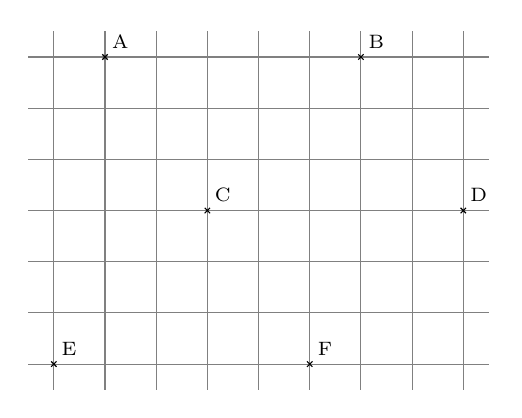
\begin{tikzpicture}[scale=0.65]
\draw [color=gray, xstep=1,ystep=1] (-0.5,-0.5) grid (8.5,6.5);
\begin{scriptsize}
\draw [color=black] (0.,0.)-- ++(-1.5pt,-1.5pt) -- ++(3.0pt,3.0pt) ++(-3.0pt,0) -- ++(3.0pt,-3.0pt);
\draw[color=black] (0.3,0.3) node {E};
\draw [color=black] (5.,0.)-- ++(-1.5pt,-1.5pt) -- ++(3.0pt,3.0pt) ++(-3.0pt,0) -- ++(3.0pt,-3.0pt);
\draw[color=black] (5.3,0.3) node {F};
\draw [color=black] (3.,3.)-- ++(-1.5pt,-1.5pt) -- ++(3.0pt,3.0pt) ++(-3.0pt,0) -- ++(3.0pt,-3.0pt);
\draw[color=black] (3.3,3.3) node {C};
\draw [color=black] (8.,3.)-- ++(-1.5pt,-1.5pt) -- ++(3.0pt,3.0pt) ++(-3.0pt,0) -- ++(3.0pt,-3.0pt);
\draw[color=black] (8.3,3.3) node {D};
\draw [color=black] (6.,6.)-- ++(-1.5pt,-1.5pt) -- ++(3.0pt,3.0pt) ++(-3.0pt,0) -- ++(3.0pt,-3.0pt);
\draw[color=black] (6.3,6.3) node {B};
\draw [color=black] (1.,6.)-- ++(-1.5pt,-1.5pt) -- ++(3.0pt,3.0pt) ++(-3.0pt,0) -- ++(3.0pt,-3.0pt);
\draw[color=black] (1.3,6.3) node {A};
\end{scriptsize}
\end{tikzpicture}}

Dire si chacune des égalités suivantes est vraie ou fausse.

\begin{multicols}{2}[\raggedcolumns]
\begin{enumerate}%[label=(\alph*)]
\item $\overrightarrow{AB}=\overrightarrow{EF}$
\item $\overrightarrow{CD}=-\overrightarrow{AB}$
\item $\overrightarrow{DA}=\overrightarrow{DB}$
\item $\overrightarrow{ED}=\overrightarrow{BD}$
\item $\overrightarrow{AE}=\overrightarrow{BF}$
\item $\overrightarrow{EF}=-\overrightarrow{DC}$
\end{enumerate}
\end{multicols}
\end{exercice}


\begin{exercice}

On considère la figure ci-dessous, formée de parallélogrammes juxtaposés.

\vspace{0.25cm}
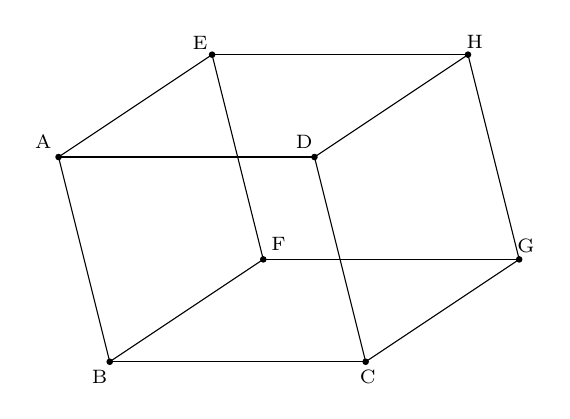
\begin{tikzpicture}[scale=0.65]
\draw (0.,4.)-- (1.,0.);
\draw (1.,0.)-- (6.,0.);
\draw (6.,0.)-- (9.,2.);
\draw (9.,2.)-- (8.,6.);
\draw (8.,6.)-- (3.,6.);
\draw (3.,6.)-- (0.,4.);
\draw (0.,4.)-- (5.,4.);
\draw (5.,4.)-- (6.,0.);
\draw (3.,6.)-- (4.,2.);
\draw (4.,2.)-- (9.,2.);
\draw (1.,0.)-- (4.,2.);
\draw (5.,4.)-- (8.,6.);
\begin{scriptsize}
\draw [fill=black] (0.,4.) circle (1.5pt);
\draw[color=black] (-0.3,4.3) node {A};
\draw [fill=black] (1.,0.) circle (1.5pt);
\draw[color=black] (0.8,-0.3) node {B};
\draw [fill=black] (6.,0.) circle (1.5pt);
\draw[color=black] (6.04,-0.3) node {C};
\draw [fill=black] (5.,4.) circle (1.5pt);
\draw[color=black] (4.8,4.3) node {D};
\draw [fill=black] (3.,6.) circle (1.5pt);
\draw[color=black] (2.767272727272728,6.2363636363636346) node {E};
\draw [fill=black] (4.,2.) circle (1.5pt);
\draw[color=black] (4.3,2.3) node {F};
\draw [fill=black] (9.,2.) circle (1.5pt);
\draw[color=black] (9.13090909090909,2.254545454545456) node {G};
\draw [fill=black] (8.,6.) circle (1.5pt);
\draw[color=black] (8.13090909090909,6.254545454545453) node {H};
\end{scriptsize}
\end{tikzpicture}

Déterminer un représentant de :

\begin{multicols}{2}[\raggedcolumns]
\begin{enumerate}%[label=(\alph*)]
\item $\overrightarrow{AE}$ ;
\item $\overrightarrow{DB}$ ;
\item $\overrightarrow{FG}$ d'origine B ;
\item $\overrightarrow{CF}$ d'extrémité E ;
\item $\overrightarrow{0}$ ;
\item $-\overrightarrow{AF}$.
\end{enumerate}
\end{multicols}

\end{exercice}

\begin{exercice}
Soit ABCD et CDEF deux parallélogrammes.\\

Montrer que ABFE est aussi un parallélogramme.
\end{exercice}

\begin{exercice}
ABCD est un rectangle de centre O.
\begin{enumerate}
\item Démontrer que $\overrightarrow{AO}=\overrightarrow{OC}$
\item Compléter en utilisant les points de la figure:
\begin{description}
\item $\overrightarrow{BO}= . . . $;
\item $\overrightarrow{CO}= . . . $;
\item $\overrightarrow{DO}= . . . $.
\end{description}
\end{enumerate}
\end{exercice}

\serie{Construction de vecteurs}

\begin{exercice}
Soit ABC un triangle quelconque.

\begin{enumerate}
\item Construire :

\begin{itemize}
\item le point N tel que $\overrightarrow{AN}=\overrightarrow{BC}$ ;
\item le point P tel que $\overrightarrow{PA}=\overrightarrow{BC}$ ;
\item le point M tel que $\overrightarrow{BM}=\overrightarrow{AC}$.
\end{itemize}

\item Montrer que A, B et C sont les milieux respectifs de $[$NP$]$, $[$PM$]$ et $[$MN$]$.

\end{enumerate}
\end{exercice}

\begin{exercice}
\begin{minipage}{0.27\linewidth}
On considère le parallélogramme ABCD représenté ci-contre.
\end{minipage}
\hspace{0.25cm}
\begin{minipage}{0.6\linewidth}
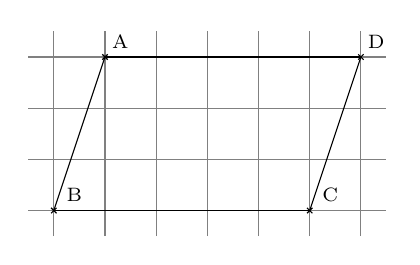
\begin{tikzpicture}[scale=0.65]
\draw [color=gray, xstep=1,ystep=1] (-0.5,-0.5) grid (6.5,3.5);
\begin{scriptsize}
\draw [color=black] (0.,0.)-- ++(-1.5pt,-1.5pt) -- ++(3.0pt,3.0pt) ++(-3.0pt,0) -- ++(3.0pt,-3.0pt);
\draw[color=black] (0.4,0.3) node {B};
\draw [color=black] (5.,0.)-- ++(-1.5pt,-1.5pt) -- ++(3.0pt,3.0pt) ++(-3.0pt,0) -- ++(3.0pt,-3.0pt);
\draw[color=black] (5.4,0.3) node {C};
\draw [color=black] (1.,3.)-- ++(-1.5pt,-1.5pt) -- ++(3.0pt,3.0pt) ++(-3.0pt,0) -- ++(3.0pt,-3.0pt);
\draw[color=black] (1.3,3.3) node {A};
\draw [color=black] (6.,3.)-- ++(-1.5pt,-1.5pt) -- ++(3.0pt,3.0pt) ++(-3.0pt,0) -- ++(3.0pt,-3.0pt);
\draw[color=black] (6.3,3.3) node {D};
\end{scriptsize}
\draw (0,0) -- (5,0);
\draw (1,3) -- (6,3);
\draw (0,0) -- (1,3);
\draw (5,0) -- (6,3);
\end{tikzpicture}
\end{minipage}

\begin{enumerate}%[label=(\alph*)]
\item Reproduire le parallélogramme ABCD sur un quadrillage.
\item Construire les points E, F, G, H et I définis par :

\begin{multicols}{2}[\raggedcolumns]
\begin{itemize}
\item $\overrightarrow{CE}=\overrightarrow{AC}$ ;
\item $\overrightarrow{CF}=\overrightarrow{AB}$ ;
\item $\overrightarrow{EG}=\overrightarrow{CD}$ ;
\item $\overrightarrow{AH}=-\overrightarrow{BC}$ ;
\item $\overrightarrow{IA}=\overrightarrow{AC}$ ;
\end{itemize}
\end{multicols}
\item Quelle est la nature des quadrilatères BCEF et DGEC ? Justifier.
\item Que représente le point A pour le segment $[$IC$]$ ? Justifier.
\end{enumerate}
\end{exercice}

\begin{exercice}
Soit ABCD un parallélogramme quelconque.
\begin{enumerate}
\item Construire le point N tel que $\overrightarrow{AN}=\overrightarrow{CB}$;
\item Que représente le point A pour le segment [DN]? Justifier;
\item Construire le point P tel que $\overrightarrow{PA}=\overrightarrow{DC}$;
\item Construire le point M tel que $\overrightarrow{BM}=\overrightarrow{AC}$;
\item Quel est la nature du quadrilatère ABMC?Justifier.
\end{enumerate}
\end{exercice}


%%%%%%%%%%%%%%%%%%%%%%%%%%%%%%%%%%%%%%%%%%%%%%%%%%%

\serie{Opérations sur les vecteurs}

\begin{exercice}
On considère la figure ci-dessous :

\vspace{0.25cm}
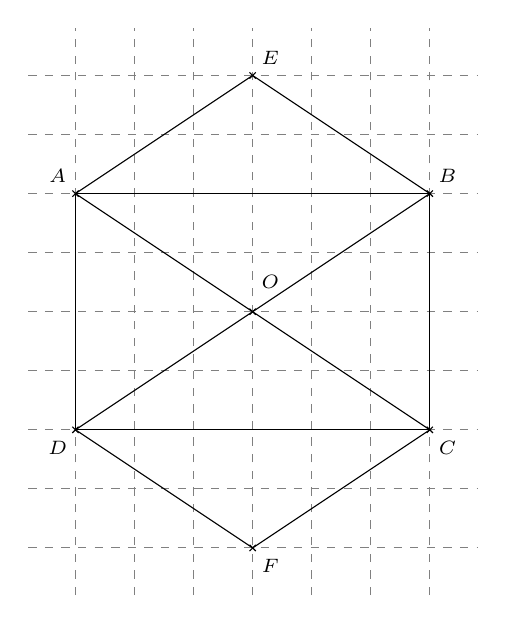
\begin{tikzpicture}[scale=0.75]
\draw [color=gray,dash pattern=on 3pt off 3pt,xstep=1,ystep=1] (-0.8,-2.8) grid (6.8,6.8);
\draw (0.,4.)-- (0.,0.);
\draw (0.,0.)-- (6.,0.);
\draw (6.,0.)-- (6.,4.);
\draw (6.,4.)-- (0.,4.);
\draw (0.,4.)-- (3.,6.);
\draw (3.,6.)-- (6.,4.);
\draw (6.,0.)-- (3.,-2.);
\draw (3.,-2.)-- (0.,0.);
\draw (0.,0.)-- (6.,4.);
\draw (0.,4.)-- (6.,0.);
\begin{scriptsize}
\draw [color=black] (0.,0.)-- ++(-1.5pt,-1.5pt) -- ++(3.0pt,3.0pt) ++(-3.0pt,0) -- ++(3.0pt,-3.0pt);
\draw[color=black] (-0.3,-0.3) node {$D$};
\draw [color=black] (6.,0.)-- ++(-1.5pt,-1.5pt) -- ++(3.0pt,3.0pt) ++(-3.0pt,0) -- ++(3.0pt,-3.0pt);
\draw[color=black] (6.3,-0.3) node {$C$};
\draw [color=black] (6.,4.)-- ++(-1.5pt,-1.5pt) -- ++(3.0pt,3.0pt) ++(-3.0pt,0) -- ++(3.0pt,-3.0pt);
\draw[color=black] (6.3,4.3) node {$B$};
\draw [color=black] (0.,4.)-- ++(-1.5pt,-1.5pt) -- ++(3.0pt,3.0pt) ++(-3.0pt,0) -- ++(3.0pt,-3.0pt);
\draw[color=black] (-0.3,4.3) node {$A$};
\draw [color=black] (3.,6.)-- ++(-1.5pt,-1.5pt) -- ++(3.0pt,3.0pt) ++(-3.0pt,0) -- ++(3.0pt,-3.0pt);
\draw[color=black] (3.3,6.3) node {$E$};
\draw [color=black] (3.,-2.)-- ++(-1.5pt,-1.5pt) -- ++(3.0pt,3.0pt) ++(-3.0pt,0) -- ++(3.0pt,-3.0pt);
\draw[color=black] (3.3,-2.3) node {$F$};
\draw [color=black] (3.,2.)-- ++(-1.5pt,-1.5pt) -- ++(3.0pt,3.0pt) ++(-3.0pt,0) -- ++(3.0pt,-3.0pt);
\draw[color=black] (3.3,2.5) node {$O$};
\end{scriptsize}
\end{tikzpicture}

\vspace{0.25cm}
Donner dans chaque cas un représentant de la somme ou de la différence des vecteurs :

\vspace{0.25cm}
\begin{itemize}
\item $\overrightarrow{AE}+\overrightarrow{AO}$ ;
\item $\overrightarrow{AE}+\overrightarrow{DF}$ ;
\item $\overrightarrow{OC}-\overrightarrow{FC}$ ;
\item $\overrightarrow{DO}+\overrightarrow{BC}+\overrightarrow{AE}$ ;
\item $\overrightarrow{BD}-\overrightarrow{BA}$.
\end{itemize}
\end{exercice}


\begin{exercice}
On considère la figure ci-dessous, formée de parallélogrammes juxtaposés.

\vspace{0.25cm}
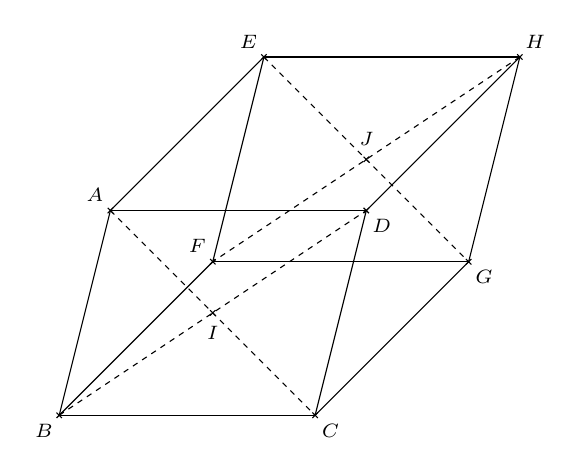
\begin{tikzpicture}[scale=0.65]
\draw (0.,0.)-- (1.,4.);
\draw (1.,4.)-- (6.,4.);
\draw (6.,4.)-- (5.,0.);
\draw (5.,0.)-- (0.,0.);
\draw [dash pattern=on 2pt off 2pt] (1.,4.)-- (5.,0.);
\draw [dash pattern=on 2pt off 2pt] (0.,0.)-- (6.,4.);
\draw (0.,0.)-- (3.,3.);
\draw (3.,3.)-- (8.,3.);
\draw (8.,3.)-- (9.,7.);
\draw (9.,7.)-- (4.,7.);
\draw (4.,7.)-- (3.,3.);
\draw [dash pattern=on 2pt off 2pt] (4.,7.)-- (8.,3.);
\draw [dash pattern=on 2pt off 2pt] (9.,7.)-- (3.,3.);
\draw (1.,4.)-- (4.,7.);
\draw (6.,4.)-- (9.,7.);
\draw (5.,0.)-- (8.,3.);
\begin{scriptsize}
\draw [color=black] (0.,0.)-- ++(-1.5pt,-1.5pt) -- ++(3.0pt,3.0pt) ++(-3.0pt,0) -- ++(3.0pt,-3.0pt);
\draw[color=black] (-0.3,-0.3) node {$B$};
\draw [color=black] (1.,4.)-- ++(-1.5pt,-1.5pt) -- ++(3.0pt,3.0pt) ++(-3.0pt,0) -- ++(3.0pt,-3.0pt);
\draw[color=black] (0.7,4.3) node {$A$};
\draw [color=black] (6.,4.)-- ++(-1.5pt,-1.5pt) -- ++(3.0pt,3.0pt) ++(-3.0pt,0) -- ++(3.0pt,-3.0pt);
\draw[color=black] (6.3,3.7) node {$D$};
\draw [color=black] (5.,0.)-- ++(-1.5pt,-1.5pt) -- ++(3.0pt,3.0pt) ++(-3.0pt,0) -- ++(3.0pt,-3.0pt);
\draw[color=black] (5.3,-0.3) node {$C$};
\draw [color=black] (3.,3.)-- ++(-1.5pt,-1.5pt) -- ++(3.0pt,3.0pt) ++(-3.0pt,0) -- ++(3.0pt,-3.0pt);
\draw[color=black] (2.7,3.3) node {$F$};
\draw [color=black] (4.,7.)-- ++(-1.5pt,-1.5pt) -- ++(3.0pt,3.0pt) ++(-3.0pt,0) -- ++(3.0pt,-3.0pt);
\draw[color=black] (3.7,7.3) node {$E$};
\draw [color=black] (9.,7.)-- ++(-1.5pt,-1.5pt) -- ++(3.0pt,3.0pt) ++(-3.0pt,0) -- ++(3.0pt,-3.0pt);
\draw[color=black] (9.3,7.3) node {$H$};
\draw [color=black] (8.,3.)-- ++(-1.5pt,-1.5pt) -- ++(3.0pt,3.0pt) ++(-3.0pt,0) -- ++(3.0pt,-3.0pt);
\draw[color=black] (8.3,2.7) node {$G$};
\draw [color=black] (3.,2.)-- ++(-1.5pt,-1.5pt) -- ++(3.0pt,3.0pt) ++(-3.0pt,0) -- ++(3.0pt,-3.0pt);
\draw[color=black] (3,1.6) node {$I$};
\draw [color=black] (6.,5.)-- ++(-1.5pt,-1.5pt) -- ++(3.0pt,3.0pt) ++(-3.0pt,0) -- ++(3.0pt,-3.0pt);
\draw[color=black] (6,5.4) node {$J$};
\end{scriptsize}
\end{tikzpicture}

\vspace{0.25cm}
Déterminer un représentant de :

\begin{multicols}{2}[\raggedcolumns]
\begin{enumerate}%[label=(\alph*)]
\item $\overrightarrow{AD}+\overrightarrow{CF}$ ;
\item $\overrightarrow{GC}+\overrightarrow{AC}$ ;
\item $\overrightarrow{HE}+\overrightarrow{BC}$ ;
\item $\overrightarrow{DE}-\overrightarrow{DH}$ ;
\item $\overrightarrow{GJ}+\overrightarrow{BF}$ ;
\item $\overrightarrow{IF}-\overrightarrow{FJ}$ ;
\item $\overrightarrow{AF}+\overrightarrow{HD}+\overrightarrow{BD}$ ;
\item $\overrightarrow{JE}+\overrightarrow{FG}-\overrightarrow{ID}$.
\end{enumerate}
\end{multicols}
\end{exercice} 


\begin{exercice}
Dans chacun des cas, construire le vecteur d’origine A égal à la somme $\overrightarrow{u}+\overrightarrow{v}$:

\begin{center}
\definecolor{yqyqyq}{rgb}{0.501960784314,0.501960784314,0.501960784314}
\begin{tikzpicture}[line cap=round,line join=round,>=triangle 45,x=1.0cm,y=1.0cm]
\draw [color=yqyqyq,dash pattern=on 4pt off 4pt, xstep=1.0cm,ystep=1.0cm] (-2.87,-0.51) grid (5.23,6.63);
\clip(-2.87,-0.51) rectangle (5.23,6.63);
\draw [->] (-2.,1.) -- (1.,5.);
\draw [->] (1.,5.) -- (4.,2.);
\begin{scriptsize}
\draw [color=black] (-2.,1.)-- ++(-1.5pt,-1.5pt) -- ++(3.0pt,3.0pt) ++(-3.0pt,0) -- ++(3.0pt,-3.0pt);
\draw[color=black] (-2.3,1.5) node {$A$};
\draw[color=black] (-0.59,3.57) node {$\overrightarrow{u}$};
\draw[color=black] (2.65,3.84) node {$\overrightarrow{v}$};
\end{scriptsize}
\end{tikzpicture}
\end{center}}
\begin{center}
\definecolor{yqyqyq}{rgb}{0.501960784314,0.501960784314,0.501960784314}
\begin{tikzpicture}[line cap=round,line join=round,>=triangle 45,x=1.0cm,y=1.0cm]
\draw [color=yqyqyq,dash pattern=on 4pt off 4pt, xstep=1.0cm,ystep=1.0cm] (-2.87,-0.51) grid (5.23,6.63);
\clip(-2.87,-0.51) rectangle (5.23,6.63);
\draw [->] (-1.,3.) -- (1.,5.);
\draw [->] (2.,6.) -- (4.,5.);
\begin{scriptsize}
\draw [color=black] (-2.,1.)-- ++(-1.5pt,-1.5pt) -- ++(3.0pt,3.0pt) ++(-3.0pt,0) -- ++(3.0pt,-3.0pt);
\draw[color=black] (-2.3,1.5) node {$A$};
\draw[color=black] (-0.26,4.32) node {$\overrightarrow{u}$};
\draw[color=black] (3.22,5.82) node {$\overrightarrow{v}$};
\end{scriptsize}
\end{tikzpicture}
\end{center}
\begin{center}
\definecolor{yqyqyq}{rgb}{0.501960784314,0.501960784314,0.501960784314}
\begin{tikzpicture}[line cap=round,line join=round,>=triangle 45,x=1.0cm,y=1.0cm]
\draw [color=yqyqyq,dash pattern=on 4pt off 4pt, xstep=1.0cm,ystep=1.0cm] (-3.77,-3.09) grid (3.19,4.05);
\clip(-3.77,-3.09) rectangle (3.19,4.05);
\draw [->] (-2.,-1.) -- (0.,-2.);
\draw [->] (2.,0.) -- (0.,-2.);
\begin{scriptsize}
\draw [color=black] (-2.,2.)-- ++(-1.5pt,-1.5pt) -- ++(3.0pt,3.0pt) ++(-3.0pt,0) -- ++(3.0pt,-3.0pt);
\draw[color=black] (-2.3,2.52) node {$A$};
\draw[color=black] (-0.89,-1.14) node {$\overrightarrow{u}$};
\draw[color=black] (0.9,-0.81) node {$\overrightarrow{v}$};
\end{scriptsize}
\end{tikzpicture}
\end{center}
\end{exercice} 

\begin{exercice}
Sur chacune des figures suivantes, construire un représentant de $\overrightarrowc{u}+\overrightarrowc{v}$ :

\begin{enumerate}
\item \ \

\begin{tikzpicture}[scale=0.75]
\draw [-latex] (0.,0.) -- (4.,1.);
\draw [-latex] (0.,0.) -- (-2.,3.);
\begin{scriptsize}
\draw [color=black,thick] (0.,0.)-- ++(-2pt,-2pt) -- ++(4pt,4pt) ++(-4pt,0) -- ++(4pt,-4pt);
\draw (2,0.5) node[below] {$\overrightarrowc{u}$};
\draw (-1,1.7) node[above] {$\overrightarrowc{v}$};
\draw [color=white] (-3,5) circle (1pt);
\draw [color=white] (0,-2) circle (1pt);
\end{scriptsize}
\end{tikzpicture}

\item \ \

\begin{tikzpicture}[scale=0.75]
\draw [-latex] (0.,0.) -- (5.,-1.);
\draw [-latex] (0.,0.) -- (-2.,0.4);
\begin{scriptsize}
\draw [color=black,thick] (0.,0.)-- ++(-2pt,-2pt) -- ++(4pt,4pt) ++(-4pt,0) -- ++(4pt,-4pt);
\draw (-1,0.2) node[above] {$\overrightarrowc{u}$};
\draw (2.5,-0.5) node[below] {$\overrightarrowc{v}$};
\draw [color=white] (-3,2.5) circle (1pt);
\draw [color=white] (0,-2.5) circle (1pt);
\end{scriptsize}
\end{tikzpicture}

\item \ \

\begin{tikzpicture}[scale=0.75]
\draw [-latex] (0.,0.) -- (2.,4.);
\draw [-latex] (-2.,-1.) -- (3.,-2.);
\begin{scriptsize}
\draw [color=black,thick] (0.,0.)-- ++(-2pt,-2pt) -- ++(4pt,4pt) ++(-4pt,0) -- ++(4pt,-4pt);
\draw [color=black,thick] (-2,-1)-- ++(-2pt,-2pt) -- ++(4pt,4pt) ++(-4pt,0) -- ++(4pt,-4pt);
\draw (0.8,2) node[above] {$\overrightarrowc{u}$};
\draw (0.5,-1.5) node[below] {$\overrightarrowc{v}$};
\draw [color=white] (-3,3) circle (1pt);
\draw [color=white] (0,-4) circle (1pt);
\end{scriptsize}
\end{tikzpicture}

\item \ \

\begin{tikzpicture}[scale=0.75]
\draw [-latex] (0.,0.) -- (-4.,1.);
\draw [-latex] (2.,2.) -- (-4.,1.);
\begin{scriptsize}
\draw [color=black,thick] (0.,0.)-- ++(-2pt,-2pt) -- ++(4pt,4pt) ++(-4pt,0) -- ++(4pt,-4pt);
\draw [color=black,thick] (2,2)-- ++(-2pt,-2pt) -- ++(4pt,4pt) ++(-4pt,0) -- ++(4pt,-4pt);
\draw (-2,0.5) node[below] {$\overrightarrowc{u}$};
\draw (-1,1.5) node[above] {$\overrightarrowc{v}$};
\draw [color=white] (-7,5) circle (1pt);
\draw [color=white] (0,-2) circle (1pt);
\end{scriptsize}
\end{tikzpicture}
\end{enumerate}
\end{exercice} 

\begin{exercice}
En utilisant la relation de Chasles, simplifier au maximum les vecteurs suivants :

\begin{enumerate}

\item $\overrightarrow{u}=\overrightarrow{AB}+\overrightarrow{BC}+\overrightarrow{CE}+\overrightarrow{EG}$
 
\item $\overrightarrow{w}=\overrightarrow{AB}+\overrightarrow{CB}+\overrightarrow{BD}+\overrightarrow{DE}$

\item $\overrightarrow{v}=\overrightarrow{AB}+\overrightarrow{DA}+\overrightarrow{CD}+\overrightarrow{BC}$ 

\item $\overrightarrow{n}=\overrightarrow{AG}+\overrightarrow{DE}+\overrightarrow{CD}+\overrightarrow{GC}$
\end{enumerate}
\end{exercice} 

\begin{exercice}
Simplifier au maximun les vecteurs suivants:
\begin{enumerate}
\item $\overrightarrow{AB}+\overrightarrow{BC}+\overrightarrow{CA}$;
\item $\overrightarrow{IJ}+\overrightarrow{KI}+\overrightarrow{JK}$;
\item $\overrightarrow{DE}+\overrightarrow{FG}+\overrightarrow{EF}-\overrightarrow{DG}$.
\end{enumerate}
\end{exercice}

\begin{exercice}
Sur chacune des figures suivantes, construire un représentant de $\overrightarrowc{u}-\overrightarrowc{v}$ :

\begin{enumerate}
\item \ \

\begin{tikzpicture}[scale=0.75]
\draw [-latex] (0.,0.) -- (4.,1.);
\draw [-latex] (0.,0.) -- (-2.,3.);
\begin{scriptsize}
\draw [color=black,thick] (0.,0.)-- ++(-2pt,-2pt) -- ++(4pt,4pt) ++(-4pt,0) -- ++(4pt,-4pt);
\draw (2,0.5) node[below] {$\overrightarrowc{u}$};
\draw (-1,1.7) node[above] {$\overrightarrowc{v}$};
\draw [color=white] (-3,5) circle (1pt);
\draw [color=white] (0,-2) circle (1pt);
\end{scriptsize}
\end{tikzpicture}

\item \ \

\begin{tikzpicture}[scale=0.75]
\draw [-latex] (0.,0.) -- (5.,-1.);
\draw [-latex] (0.,0.) -- (-2.,0.4);
\begin{scriptsize}
\draw [color=black,thick] (0.,0.)-- ++(-2pt,-2pt) -- ++(4pt,4pt) ++(-4pt,0) -- ++(4pt,-4pt);
\draw (-1,0.2) node[above] {$\overrightarrowc{u}$};
\draw (2.5,-0.5) node[below] {$\overrightarrowc{v}$};
\draw [color=white] (-3,2.5) circle (1pt);
\draw [color=white] (0,-2.5) circle (1pt);
\end{scriptsize}
\end{tikzpicture}

\item \ \

\begin{tikzpicture}[scale=0.75]
\draw [-latex] (0.,0.) -- (2.,4.);
\draw [-latex] (-2.,-1.) -- (3.,-2.);
\begin{scriptsize}
\draw [color=black,thick] (0.,0.)-- ++(-2pt,-2pt) -- ++(4pt,4pt) ++(-4pt,0) -- ++(4pt,-4pt);
\draw [color=black,thick] (-2,-1)-- ++(-2pt,-2pt) -- ++(4pt,4pt) ++(-4pt,0) -- ++(4pt,-4pt);
\draw (0.8,2) node[above] {$\overrightarrowc{u}$};
\draw (0.5,-1.5) node[below] {$\overrightarrowc{v}$};
\draw [color=white] (-3,3) circle (1pt);
\draw [color=white] (0,-4) circle (1pt);
\end{scriptsize}
\end{tikzpicture}

\item \ \

\begin{tikzpicture}[scale=0.75]
\draw [-latex] (0.,0.) -- (-4.,1.);
\draw [-latex] (2.,2.) -- (-4.,1.);
\begin{scriptsize}
\draw [color=black,thick] (0.,0.)-- ++(-2pt,-2pt) -- ++(4pt,4pt) ++(-4pt,0) -- ++(4pt,-4pt);
\draw [color=black,thick] (2,2)-- ++(-2pt,-2pt) -- ++(4pt,4pt) ++(-4pt,0) -- ++(4pt,-4pt);
\draw (-2,0.5) node[below] {$\overrightarrowc{u}$};
\draw (-1,1.5) node[above] {$\overrightarrowc{v}$};
\draw [color=white] (-7,5) circle (1pt);
\draw [color=white] (0,-2) circle (1pt);
\end{scriptsize}
\end{tikzpicture}
\end{enumerate}
\end{exercice} 

\begin{exercice}
Reproduire chacune des figures suivantes, puis construire le vecteur demandé :

\vspace{0.25cm}
\renewcommand{\arraystretch}{0.6}
\begin{tabular}{m{0.2cm}ll}
1. & \ 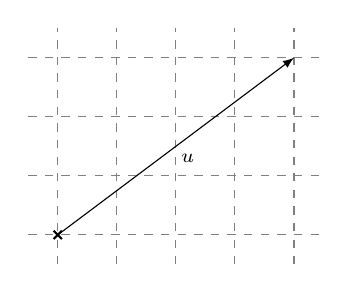
\begin{tikzpicture}[scale=0.75]
\draw [color=gray,dash pattern=on 3pt off 3pt,xstep=1,ystep=1] (-0.5,-0.5) grid (4.5,3.5);
\draw [-latex] (0,0) -- (4,3);
\begin{scriptsize}
\draw [color=black,thick] (0.,0.)-- ++(-2pt,-2pt) -- ++(4pt,4pt) ++(-4pt,0) -- ++(4pt,-4pt);
\draw (2.2,1.5) node[below] {$\overrightarrowc{u}$};
\end{scriptsize}
\end{tikzpicture}
& $2,5\overrightarrowc{u}$ ;\\
&&\\
2. & \ 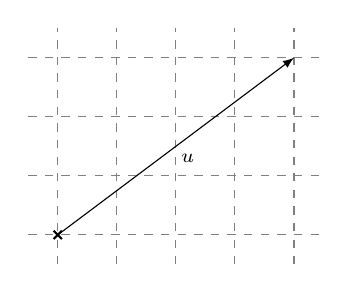
\begin{tikzpicture}[scale=0.75]
\draw [color=gray,dash pattern=on 3pt off 3pt,xstep=1,ystep=1] (-0.5,-0.5) grid (4.5,3.5);
\draw [-latex] (0,0) -- (4,3);
\begin{scriptsize}
\draw [color=black,thick] (0.,0.)-- ++(-2pt,-2pt) -- ++(4pt,4pt) ++(-4pt,0) -- ++(4pt,-4pt);
\draw (2.2,1.5) node[below] {$\overrightarrowc{u}$};
\end{scriptsize}
\end{tikzpicture}
& $-\dfrac{3}{4}\overrightarrowc{u}$ ;\\
&&\\
3. & \ 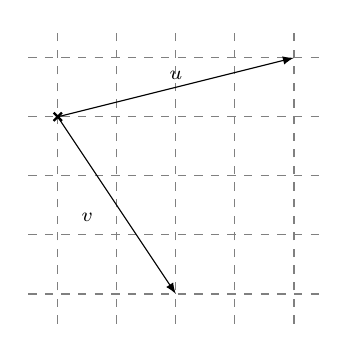
\begin{tikzpicture}[scale=0.75]
\draw [color=gray,dash pattern=on 3pt off 3pt,xstep=1,ystep=1] (-0.5,-1.5) grid (4.5,3.5);
\draw [-latex] (0,2) -- (4,3);
\draw [-latex] (0,2) -- (2,-1);
\draw [color=black,thick] (0,2)-- ++(-2pt,-2pt) -- ++(4pt,4pt) ++(-4pt,0) -- ++(4pt,-4pt);
\begin{scriptsize}
\draw (2,2.5) node[above] {$\overrightarrowc{u}$};
\draw (0.5,0.5) node[below] {$\overrightarrowc{v}$};
\end{scriptsize}
\end{tikzpicture}
& $3\overrightarrowc{u}-2\overrightarrowc{v}$ ;\\
&&\\
4. & \ 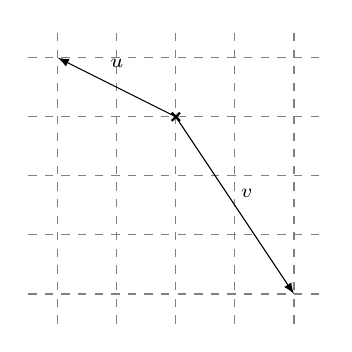
\begin{tikzpicture}[scale=0.75]
\draw [color=gray,dash pattern=on 3pt off 3pt,xstep=1,ystep=1] (-0.5,-1.5) grid (4.5,3.5);
\draw [-latex] (2,2) -- (0,3);
\draw [-latex] (2,2) -- (4,-1);
\draw [color=black,thick] (2,2)-- ++(-2pt,-2pt) -- ++(4pt,4pt) ++(-4pt,0) -- ++(4pt,-4pt);
\begin{scriptsize}
\draw (1,2.7) node[above] {$\overrightarrowc{u}$};
\draw (3.2,0.5) node[above] {$\overrightarrowc{v}$};
\end{scriptsize}
\end{tikzpicture}
& $-\dfrac{5}{2}\overrightarrowc{u}+\dfrac{2}{3}\overrightarrowc{v}$ ;\\
\end{tabular}
\end{exercice} 

\begin{exercice}
Construire le vecteur d’origine A égale à $3\overrightarrow{u}+2\overrightarrow{v}$.

\begin{tikzpicture}[line cap=round,line join=round,>=triangle 45,x=1.0cm,y=1.0cm]
\clip(-3.77,-2.7) rectangle (5.2,4.95);
\draw [->] (-2.,-1.) -- (0.,-2.);
\draw [->] (1.18,-2.19) -- (2.44,-1.14);
\begin{scriptsize}
\draw [color=black] (-2.,3.)-- ++(-1.5pt,-1.5pt) -- ++(3.0pt,3.0pt) ++(-3.0pt,0) -- ++(3.0pt,-3.0pt);
\draw[color=black] (-2.3,3.51) node {$A$};
\draw[color=black] (-0.89,-1.14) node {$\overrightarrow{u}$};
\draw[color=black] (1.57,-1.32) node {$\overrightarrow{v}$};
\end{scriptsize}
\end{tikzpicture}
\end{exercice} 

\begin{exercice}
Construire le vecteur d’origine A égale à $\overrightarrow{u}-2\overrightarrow{v}$.

\begin{tikzpicture}[line cap=round,line join=round,>=triangle 45,x=1.0cm,y=1.0cm]
\clip(-4.82,-2.73) rectangle (4.15,4.92);
\draw [->] (-2.,-1.) -- (0.,-2.);
\draw [->] (1.18,-2.19) -- (2.44,-1.14);
\begin{scriptsize}
\draw [color=black] (-2.,3.)-- ++(-1.5pt,-1.5pt) -- ++(3.0pt,3.0pt) ++(-3.0pt,0) -- ++(3.0pt,-3.0pt);
\draw[color=black] (-2.3,3.51) node {$A$};
\draw[color=black] (-0.89,-1.14) node {$\overrightarrow{u}$};
\draw[color=black] (1.57,-1.32) node {$\overrightarrow{v}$};
\end{scriptsize}
\end{tikzpicture}
\end{exercice}

\begin{exercice}
Construire les points M, N, et P définis par : $\overrightarrow{AM}=\dfrac{2}{3}\overrightarrow{u}$; $\overrightarrow{AN}=-2\overrightarrow{v}$  et $\overrightarrow{BP}=-\dfrac{1}{3}\overrightarrow{u}+\overrightarrow{v}$ .\\

\definecolor{yqyqyq}{rgb}{0.501960784314,0.501960784314,0.501960784314}
\begin{tikzpicture}[line cap=round,line join=round,>=triangle 45,x=1.0cm,y=1.0cm]
\draw [color=yqyqyq,dash pattern=on 4pt off 4pt, xstep=1.0cm,ystep=1.0cm] (-5.84,-0.93) grid (2.62,6.72);
\clip(-5.84,-0.93) rectangle (2.62,6.72);
\draw [->] (-5.,3.) -- (-2.,6.);
\draw [->] (0.,0.) -- (-2.,1.);
\begin{scriptsize}
\draw [color=black] (-2.,3.)-- ++(-1.5pt,-1.5pt) -- ++(3.0pt,3.0pt) ++(-3.0pt,0) -- ++(3.0pt,-3.0pt);
\draw[color=black] (-2.3,3.51) node {$A$};
\draw[color=black] (-3.65,4.86) node {$\overrightarrow{u}$};
\draw[color=black] (-0.74,0.78) node {$\overrightarrow{v}$};
\draw [color=black] (1.,5.)-- ++(-1.5pt,-1.5pt) -- ++(3.0pt,3.0pt) ++(-3.0pt,0) -- ++(3.0pt,-3.0pt);
\draw[color=black] (1.21,5.43) node {$B$};
\end{scriptsize}
\end{tikzpicture}
\end{exercice}

\begin{exercice}
Simplifier au maximun les vecteurs suivants:
\begin{enumerate}
\item $\overrightarrow{AE}+\overrightarrow{FT}+\overrightarrow{KA}+\overrightarrow{EF}$ ;
\item $\overrightarrow{AB}-\overrightarrow{AC}-\overrightarrow{CB}$ ;
\item $\overrightarrow{AC}+2\overrightarrow{CB}+\overrightarrow{BA}$ ;
\item $-\overrightarrow{HD}+\overrightarrow{ZA}+\overrightarrow{HR}-\overrightarrow{DN}+\overrightarrow{RZ}$ ;
\item $3\overrightarrow{AB}+2\overrightarrow{BC}+4\overrightarrow{CA}$ ;
\item $\overrightarrow{AB}-2\overrightarrow{AC}+2\overrightarrow{BC}$.
\end{enumerate}
\end{exercice}







\end{colonne*exercice}




\connaissances


\QCMautoevaluation{Pour chaque question, plusieurs réponses sont
  proposées.  Déterminer celles qui sont correctes.}


\begin{QCM}

\begin{GroupeQCM}

\begin{center}
\begin{tikzpicture}[scale=0.8][general]
 \draw (0,0)--(1,3)--(3,3)--(2,0)--cycle;
 \draw (1,3)--(3,0)--(5,-0.3)--(3,3);
 \draw (0,0)node[left] {$F$};
 \draw (1,3)node[above] {$A$};
 \draw (3,3)node[above] {$B$};
 \draw (2,0)node[below] {$C$};
 \draw (5,-0.3)node[below] {$D$};
 \draw (3,0)node[below] {$E$};
 \draw[color=C1] (0.5,1.5)node {{\boldmath $\infty$}};
 \draw[color=C1] (2.5,1.5)node {{\boldmath $\infty$}};
 \draw[color=F1] (2,3)node[rotate=90] {{\boldmath $\approx$}};
 \draw[color=F1] (1,0)node[rotate=90] {{\boldmath $\approx$}};
 \draw[color=F1] (4,-0.1)node[rotate=90] {{\boldmath $\approx$}};
\end{tikzpicture}
\end{center}

\begin{exercice}L'image de $F$ dans la translation de vecteur $\vv{AB}$ est le point:
\begin{ChoixQCM}{2}
\item $C$
\item $E$
\end{ChoixQCM}
\begin{corrige}
\reponseQCM{a}
\end{corrige}
\end{exercice}

\begin{exercice}$\vv{AB}+\vv{BD}=\vv{AD}$
\begin{ChoixQCM}{2}
\item vrai
\item faux
\end{ChoixQCM}
\begin{corrige}
\reponseQCM{a}
\end{corrige}
\end{exercice}

\begin{exercice}$AB+BD=AD$
\begin{ChoixQCM}{2}
\item vrai
\item faux
\end{ChoixQCM}
\begin{corrige}
\reponseQCM{b}
\end{corrige}
\end{exercice}

\begin{exercice}$ABDE$ est un parallélogramme.
\begin{ChoixQCM}{2}
\item vrai
\item faux
\end{ChoixQCM}
\begin{corrige}
\reponseQCM{b}
\end{corrige}
\end{exercice}

\begin{exercice}$FCBA$ est un parallélogramme.
\begin{ChoixQCM}{2}
\item vrai
\item faux
\end{ChoixQCM}
\begin{corrige}
\reponseQCM{a}
\end{corrige}
\end{exercice}


\begin{exercice}$\vv{AB}=\vv{CF}$
\begin{ChoixQCM}{2}
\item vrai
\item faux
\end{ChoixQCM}
\begin{corrige}
\reponseQCM{b}
\end{corrige}
\end{exercice}

\begin{exercice}$\vv{DE}=\vv{BA}$
\begin{ChoixQCM}{2}
\item vrai
\item faux
\end{ChoixQCM}
\begin{corrige}
\reponseQCM{b}
\end{corrige}
\end{exercice}

\begin{exercice}$DE=BA$
\begin{ChoixQCM}{2}
\item vrai
\item faux
\end{ChoixQCM}
\begin{corrige}
\reponseQCM{a}
\end{corrige}
\end{exercice}

\begin{exercice}$\vv{AB}+\vv{AF}=\vv{AC}$
\begin{ChoixQCM}{2}
\item vrai
\item faux
\end{ChoixQCM}
\begin{corrige}
\reponseQCM{a}
\end{corrige}
\end{exercice}

\begin{exercice}$\vv{CB}+\vv{AB}=\vv{CA}$
\begin{ChoixQCM}{2}
\item vrai
\item faux
\end{ChoixQCM}
\begin{corrige}
\reponseQCM{b}
\end{corrige}
\end{exercice}



\end{GroupeQCM}
\end{QCM}

  




\pagebreak





\themaC
\chapter{Les racines carrées }\label{ChLesRacinesCarrees}

\begin{acquis}
\begin{itemize}
\item Savoir simplifier des expressions comportant des racines carrées;
\item Savoir éliminer les radicaux aux dénominateurs des fractions.
\end{itemize}
\end{acquis}


\exercicesbase
\begin{colonne*exercice}

\begin{center}

\includegraphics[scale=0.2]{no_calculator}
\end{center}

\serie{Racines et opérations}



\begin{exercice}
\begin{enumerate}
\item Ecrire les nombres ci-dessous sous la forme $a \sqrt{2}$  où $a$ désigne un nombre entier. On détaillera les étapes.\\

\begin{tabular}{m{3.8cm}m{3.5cm}}
A = $\sqrt{8}$ & B = $\sqrt{32}$\\
&\\
C = $\sqrt{200}$ & D = $2\sqrt{18}$\\
&\\

\end{tabular}

\item Ecrire les nombres ci-dessous sous la forme $a \sqrt{3}$  où $a$ désigne un nombre entier. On détaillera les étapes.

\begin{tabular}{m{3.8cm}m{3.5cm}}
E = $\sqrt{12}$ & F = $\sqrt{75}$\\
&\\
G = $5\sqrt{48}$ & H = $-10\sqrt{27}$\\
&\\

\end{tabular}

\item Ecrire les nombres ci-dessous sous la forme $a \sqrt{b}$  où $a$ et $b$ sont deux entiers avec $b$ le plus petit possible. On détaillera les étapes.

\begin{tabular}{m{3.8cm}m{3.5cm}}
I = $\sqrt{108}$ & J = $\sqrt{128}$\\
&\\
K = $3\sqrt{24}$ & L = $5\sqrt{98}$\\
&\\
M = $-3\sqrt{180}$ &\\
&\\
\end{tabular}
\end{enumerate}

\end{exercice}


\begin{exercice}

Réduire les sommes suivantes:\\

A = $\sqrt{50}+3\sqrt{2}$\\

B = $5\sqrt{3}-\sqrt{12}$\\

C = $\sqrt{20}+4\sqrt{5}-8\sqrt{45}$\\

D = $-7\sqrt{24}+2\sqrt{54}-\sqrt{150}$\\
\end{exercice}


\begin{exercice}

Réduire les sommes suivantes:\\

A = $\sqrt{8}+\sqrt{18}+\sqrt{50}$\\

B = $3\sqrt{5}+4\sqrt{125}-7\sqrt{45}$\\

C = $\sqrt{40}-2\sqrt{250}-\sqrt{160}$\\

D = $\sqrt{28}+\sqrt{63}-\sqrt{700}+\sqrt{112}$\\

\end{exercice}

\begin{exercice}
Montrer que les nombres suivants sont des entiers:\\

\begin{tabular}{m{3.8cm}m{3.5cm}}
A = $\dfrac{\sqrt{45}}{\sqrt{5}}$ & B = $\dfrac{\sqrt{128}}{\sqrt{32}}$\\
&\\
C = $\sqrt{3} \times \sqrt{12}$ & D = $\sqrt{48} \times \sqrt{\dfrac{1}{3}}$\\
&\\
E = $\dfrac{4\sqrt{7}}{\sqrt{28}}$ & F = $8\sqrt{15} \sqrt{\dfrac{3}{5}}$\\
&\\


\end{tabular}
\end{exercice}

\begin{exercice}
Sans utiliser de valeurs approchées, montrer que trois de ces nombres sont égaux:\\

\begin{tabular}{m{3.8cm}m{3.5cm}}
A = $\sqrt{5}+\sqrt{5}$ & B = $\dfrac{\sqrt{500}}{5}$\\
&\\
C = $2\sqrt{5} \sqrt{5}$ & D = $\sqrt{5+5}$\\
&\\
E = $\sqrt{20}$ &\\
&\\


\end{tabular}
\end{exercice}

\begin{exercice}

Ecrire les expressions ci-dessous sous la forme $a \sqrt{b}$  où $a$ et $b$ sont deux entiers avec $b$ le plus petit possible.\\

\begin{tabular}{m{3.8cm}m{3.5cm}}
A = $5\sqrt{6} \times 2\sqrt{3}$ & B = $\sqrt{75}+7\sqrt{3}-2\sqrt{27}$\\
&\\
C = $\sqrt{6} \times \sqrt{42}$ &\\
&\\

\end{tabular}

D = $2\sqrt{18}-3\sqrt{50}+100\sqrt{2}$ \\
\end{exercice}

\serie{Racines et dénominateurs}

\begin{exercice}
Transformer les écritures suivantes pour obtenir un dénominateur entier:\\

\begin{tabular}{m{3.8cm}m{3.5cm}}
A = $\dfrac{5}{\sqrt{7}}$ & B = $-\dfrac{8}{\sqrt{13}}$\\
&\\
C = $\dfrac{3}{\sqrt{6}}$ & D = $\dfrac{4}{3\sqrt{3}}$\\
&\\
E = $\dfrac{2-\sqrt{2}}{\sqrt{2}}$ &\\
&\\


\end{tabular}
\end{exercice}

\begin{exercice}
Transformer les écritures suivantes pour obtenir un dénominateur entier:\\

\begin{tabular}{m{3.8cm}m{3.5cm}}
A = $\dfrac{3}{\sqrt{2}+1}$ & B = $\dfrac{7}{\sqrt{3}-2}$\\
&\\
C = -$\dfrac{\sqrt{7}}{6+\sqrt{7}}$ & D = $\dfrac{\sqrt{5}+1}{\sqrt{5}-1}$\\
&\\
E = $\dfrac{3-\sqrt{11}}{4+\sqrt{11}}$ &\\
&\\

\end{tabular}

\end{exercice}

%%%%%%%%%%%%%%%%%%%%%%%%%%%%%%%%%%%%%%%%%%%%%%%%%%%

\serie{Divers}

\begin{exercice}
On considère un carré de côté $\sqrt{3} + 3$ cm 

et un rectangle dont les  dimensions  sont:

 $\sqrt{72}+ 3\sqrt{6}$ cm  et $\sqrt{2}$ cm .

Démontrer que ce carré et ce rectangle ont la même aire.
\end{exercice}


\begin{exercice}
Le tableau ci-dessous est-il un tableau de proportionnalité?

Justifier votre réponse.
%\begin{center}
%\includegraphics[scale=0.5]{R2}
%\end{center}
\end{exercice} 


\begin{exercice}
Soit P le nombre défini par : P = $\left( 2 \sqrt{5}+\sqrt{8}\right) ^2$.

\begin{enumerate}
\item Ecrire P sous la forme $a+b\sqrt{c}$ où $a$, $b$ et $c$ sont des entiers, $c$ le plus petit possible.
\item Quel nombre positif a pour carré $59+30\sqrt{2}$?
\end{enumerate}
\end{exercice} 

\begin{exercice}

\begin{enumerate}
\item Démontrer que $\sqrt{48}+\sqrt{108}=\sqrt{300}$.
\item Démontrer que $4\sqrt{18} \times \sqrt{24}=48\sqrt{3}$.
\end{enumerate}
\end{exercice} 

\begin{exercice}
On considère les nombres suivants:

A = $2\sqrt{27}-2\sqrt{3}+\sqrt{12}$ et 

B = $\sqrt{75}+\sqrt{48}-7\sqrt{3}$.

Montrer en détaillant les calculs que $\dfrac{\text{A}}{\text{B}}$ est un nombre entier.
\end{exercice} 









\end{colonne*exercice}




\connaissances


\QCMautoevaluation{Pour chaque question, plusieurs réponses sont
  proposées.  Déterminer celles qui sont correctes.}


\begin{QCM}

\begin{GroupeQCM}

\begin{exercice}$(-3\sqrt{5})^2$ est égal à ...
\begin{ChoixQCM}{3}
\item $-15$
\item $45$
\item $30$
\end{ChoixQCM}
\begin{corrige}
\reponseQCM{6}
\end{corrige}
\end{exercice}

\begin{exercice}$\dfrac{\sqrt{80}}{2}$ s'écrit aussi ...
\begin{ChoixQCM}{3}
\item $2\sqrt{10}$
\item $2\sqrt{5}$
\item $\sqrt{20}$
\end{ChoixQCM}
\begin{corrige}
\reponseQCM{b c}
\end{corrige}
\end{exercice}

\begin{exercice}$3\sqrt{2}+\sqrt{8}$ est égal à ...
\begin{ChoixQCM}{3}
\item $5\sqrt{2}$
\item $3\sqrt{10}$
\item Ne se réduit pas
\end{ChoixQCM}
\begin{corrige}
\reponseQCM{a}
\end{corrige}
\end{exercice}

\begin{exercice}$5\sqrt{3} \times 2\sqrt{3}$ est égal à ...
\begin{ChoixQCM}{3}
\item $10\sqrt{3}$
\item $30$
\item Ne se réduit pas
\end{ChoixQCM}
\begin{corrige}
\reponseQCM{b}
\end{corrige}
\end{exercice}

\end{GroupeQCM}
\end{QCM}

  




\pagebreak





%\themaG
%\chapter{Les théorèmes en géométrie}\label{ChLesTheoremes}

\begin{acquis}
\begin{itemize}
\item Savoir utiliser le théorème de Pythagore, sa réciproque et sa contraposée;
\item Savoir utiliser le théorème de Thalès, sa réciproque et sa contraposée.
\end{itemize}
\end{acquis}



\exercicesbase
\begin{colonne*exercice}

\serie{Théorème de Pythagore}

\begin{exercice}
Pour chacun des triangles suivants, calculer la longueur du troisième côté.

Si nécessaire, arrondir le résultat au millimètre.

\begin{enumerate}
\item ABC est un triangle rectangle en A tel que

AB = 4,5 cm et AC = 6 cm.
\item MER est un triangle rectangle en E tel que

MR = 6,5 cm et ME = 3,9 cm.
\item ART est un triangle rectangle en T tel que

AT = 7 cm et AR = 11 cm.
\end{enumerate}

\end{exercice}


\begin{exercice}
Sur la figure, qui n’est pas en vraie grandeur : AB = 1,5 cm ; AD = 6 cm et  BC = 12 cm.

\begin{minipage}{0.6\linewidth}

\begin{enumerate}
\item Calculer la valeur arrondie au mm de BD.

\item Calculer, en justifiant, la valeur exacte de DC.\\\\

\end{enumerate}

\end{minipage}
\hfill
\begin{minipage}{0.3\linewidth}
\begin{center}
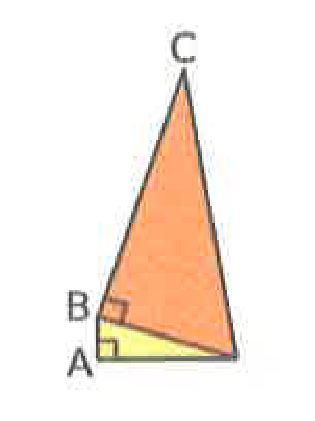
\includegraphics[scale=0.5]{T1}
\end{center}
\end{minipage}
\end{exercice}


\begin{exercice}
Après un violent orage, Julia constate que la foudre a cassé son arbre préféré à 2 m du sol.

La cime touche le sol à 7 m du pied de l’arbre.

\begin{center}
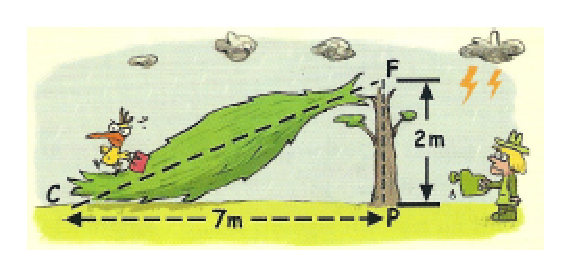
\includegraphics[scale=0.55]{T7}
\end{center}
Quelle était la hauteur de l'arbre avant l'orage, au décimètre près ?

\end{exercice}

\begin{exercice}
\emph{On considère le triangle \emph{BEA} représenté ci-dessous :}

\vspace{0,25cm}

\begin{center}
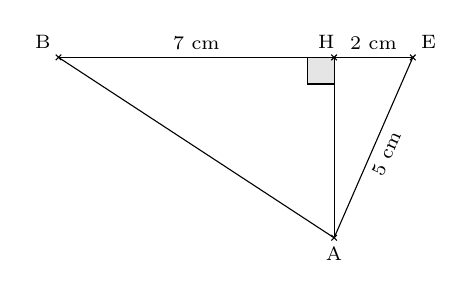
\begin{tikzpicture}[x=0.5cm,y=0.5cm]
\draw[fill=black,fill opacity=0.1] (6.324340988406047,-8.274436458635991E-17) -- (6.324340988406047,-0.6756590115939533) -- (7.0,-0.6756590115939531) -- (7.0,0.0) -- cycle; 
\draw (0.0,-0.0)-- (7.0,0.0);
\draw (7.0,0.0)-- (9.0,0.0);
\draw (9.0,0.0)-- (7.0,-4.58257569495584);
\draw (7.0,-4.58257569495584)-- (7.0,0.0);
\draw (7.0,-4.58257569495584)-- (0.0,-0.0);
\begin{scriptsize}
\draw [color=black] (0.0,-0.0)-- ++(-1.0pt,-1.0pt) -- ++(2.0pt,2.0pt) ++(-2.0pt,0) -- ++(2.0pt,-2.0pt);
\draw[color=black] (-0.4,0.4) node {B};
\draw [color=black] (7.0,0.0)-- ++(-1.0pt,-1.0pt) -- ++(2.0pt,2.0pt) ++(-2.0pt,0) -- ++(2.0pt,-2.0pt);
\draw[color=black] (6.8,0.4) node {H};
\draw [color=black] (9.0,0.0)-- ++(-1.0pt,-1.0pt) -- ++(2.0pt,2.0pt) ++(-2.0pt,0) -- ++(2.0pt,-2.0pt);
\draw[color=black] (9.4,0.4) node {E};
\draw [color=black] (7.0,-4.58257569495584)-- ++(-1.0pt,-1.0pt) -- ++(2.0pt,2.0pt) ++(-2.0pt,0) -- ++(2.0pt,-2.0pt);
\draw[color=black] (7,-5) node {A};
\draw (3.5,0) node[above] {7 cm};
\draw (8,0) node[above] {2 cm};
\draw (8,-2.3) node[below,rotate=66] {5 cm};
\end{scriptsize}
\end{tikzpicture}
\end{center}

\begin{enumerate}
\item Calculer l'aire du triangle BEA, arrondie au mm$^2$. On détaillera les étapes du raisonnement.
\item Calculer la longueur AB. Donner sa valeur exacte et sa valeur arrondie au mm.
\end{enumerate}
\end{exercice}

\begin{exercice}
Un triangle $EFG$ est rectangle en $E$ avec $EG = 7 cm$ et $\widehat{FGE} = 45°$.
\begin{enumerate}
\item Calculer la mesure de l'angle  $\widehat{EFG}$.
\item Calculer, en justifiant, $EF$ et $FG$ (arrondir au mm).
\end{enumerate}
\end{exercice}

\begin{exercice}
Rectangle ou non ?
\begin{enumerate}
\item Le triangle XYZ est tel que  XY =29,8cm ; YZ = 28,1cm et  XZ= 10,2cm.\\
Est-il rectangle ? Justifier.
\item Soit le triangle ALE tel que :	AL = 13,1cm ; LE = 11,2cm ; EA = 6,6 cm.\\
Est-il rectangle ? Justifier.
\end{enumerate}
\end{exercice}

\begin{exercice}
Pour chacun des triangles suivants, déterminer s'il s'agit ou non d'un triangle rectangle et préciser, le cas échéant, quelle est son hypoténuse.

\begin{enumerate}
\item TOP \emph{est un triangle tel que}

OT = 39 cm, OP = 65 cm \emph{et} TP = 52 cm.

\vspace{0.25cm}
\item BUS \emph{est un triangle tel que}

BU = 8 cm, US = 4,5 cm \emph{et} BS = 9,2 cm.
\end{enumerate}
\end{exercice}

\begin{exercice}
On considère le  parallélogramme STOP dessiné à main levée.\\
\begin{minipage}{0.6\linewidth}


Démontrer que le parallélogramme STOP est un rectangle.

\end{minipage}
\hfill
\begin{minipage}{0.3\linewidth}
\begin{center}
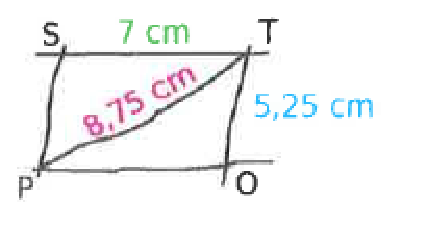
\includegraphics[scale=0.5]{T2}
\end{center}
\end{minipage}
\end{exercice}

\begin{exercice}
Sur la figure ci-contre :

\begin{minipage}{0.6\linewidth}
\begin{itemize}
\item EFGH \emph{est un rectangle} ;
\item EF = 14 m \emph{et} FG = 12 m ;
\item K $\in$ [EH] \emph{et} EK = 4 m ;
\item L $\in$ [EF] \emph{et} EL = 6 m.
\end{itemize}
Le triangle KGL est-il rectangle ?

\end{minipage}
\hfill
\begin{minipage}{0.3\linewidth}
\begin{center}

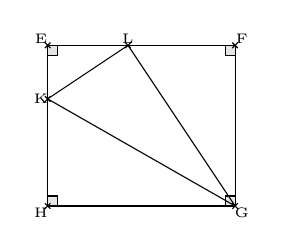
\begin{tikzpicture}[x=0.17cm,y=0.17cm]
\draw[fill=black,fill opacity=0.1] (0.7415589313755807,0.0) -- (0.7415589313755808,0.7415589313755807) -- (4.540738858441183E-17,0.7415589313755807) -- (0.0,-0.0) -- cycle; 
\draw[fill=black,fill opacity=0.1] (13.25844106862442,12.0) -- (13.25844106862442,11.25844106862442) -- (14.0,11.25844106862442) -- (14.0,12.0) -- cycle; 
\draw[fill=black,fill opacity=0.1] (4.540738858441183E-17,11.25844106862442) -- (0.7415589313755808,11.25844106862442) -- (0.7415589313755807,12.0) -- (0.0,12.0) -- cycle; 
\draw[fill=black,fill opacity=0.1] (14.0,0.7415589313755807) -- (13.25844106862442,0.7415589313755808) -- (13.25844106862442,9.081477716882366E-17) -- (14.0,0.0) -- cycle; 
\draw (0.0,-0.0)-- (0.0,12.0);
\draw (0.0,12.0)-- (14.0,12.0);
\draw (14.0,12.0)-- (14.0,0.0);
\draw (14.0,0.0)-- (0.0,-0.0);
\draw (0.0,8.0)-- (6.0,12.0);
\draw (6.0,12.0)-- (14.0,0.0);
\draw (14.0,0.0)-- (0.0,8.0);
\begin{tiny}
\draw [color=black] (0.0,-0.0)-- ++(-1.0pt,-1.0pt) -- ++(2.0pt,2.0pt) ++(-2.0pt,0) -- ++(2.0pt,-2.0pt);
\draw[color=black] (-0.5,-0.5) node {H};
\draw [color=black] (14.0,0.0)-- ++(-1.0pt,-1.0pt) -- ++(2.0pt,2.0pt) ++(-2.0pt,0) -- ++(2.0pt,-2.0pt);
\draw[color=black] (14.5,-0.5) node {G};
\draw [color=black] (0.0,12.0)-- ++(-1.0pt,-1.0pt) -- ++(2.0pt,2.0pt) ++(-2.0pt,0) -- ++(2.0pt,-2.0pt);
\draw[color=black] (-0.5,12.5) node {E};
\draw [color=black] (14.0,12.0)-- ++(-1.0pt,-1.0pt) -- ++(2.0pt,2.0pt) ++(-2.0pt,0) -- ++(2.0pt,-2.0pt);
\draw[color=black] (14.5,12.5) node {F};
\draw [color=black] (0.0,8.0)-- ++(-1.0pt,-1.0pt) -- ++(2.0pt,2.0pt) ++(-2.0pt,0) -- ++(2.0pt,-2.0pt);
\draw[color=black] (-0.5,8) node {K};
\draw [color=black] (6.0,12.0)-- ++(-1.0pt,-1.0pt) -- ++(2.0pt,2.0pt) ++(-2.0pt,0) -- ++(2.0pt,-2.0pt);
\draw[color=black] (6,12.5) node {L};
\end{tiny}
\end{tikzpicture}
\end{center}
\end{minipage}
\end{exercice}

\newpage

\serie{Théorème de Thalès}

\begin{exercice}
Sur la figure ci-dessous, les droites (LN) et (RO) sont paralléles (les longueurs sont en centimètres).

Les droites (RN) et (OA) sont sécantes en L.

Calculer les longueurs LR et AO.


\begin{center}
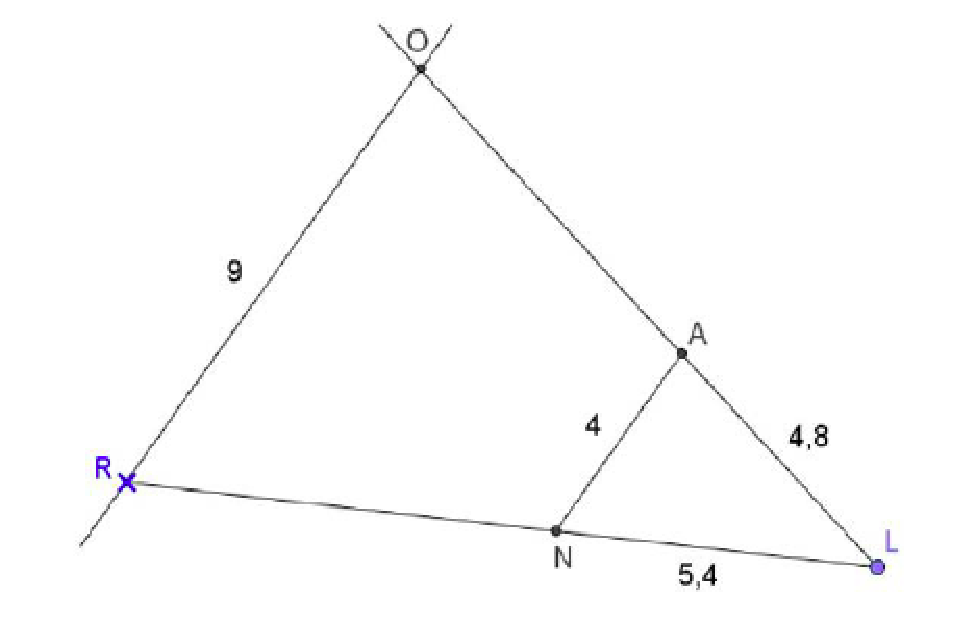
\includegraphics[scale=0.4]{T8}
\end{center}
\end{exercice}

\begin{exercice}
On suppose que $(AB)\parallel (CD)$, $AB = 72$, $CD = 96$, $SC = 84$ et $SD = 72$. Les mesures sont en millimètres.

\begin{center}
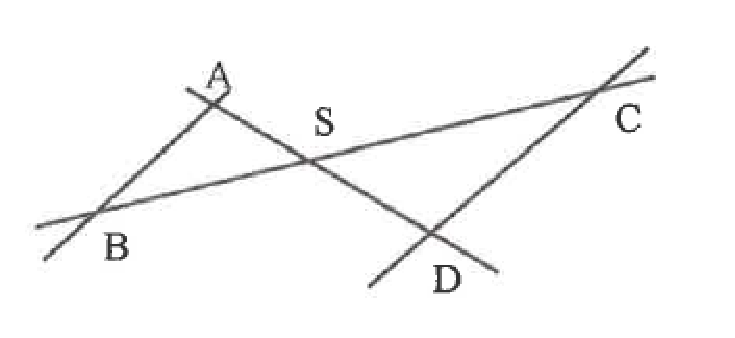
\includegraphics[scale=0.5]{T3}
\end{center}

Trouver $SA$ et $SB$.
\end{exercice}

\begin{exercice}
Lors de son premier voyage en Egypte, Thalès applique le théorème qui porte aujourd'hui son nom pour mesurer la hauteur de la grande pyramide de Kheops.

\begin{center}
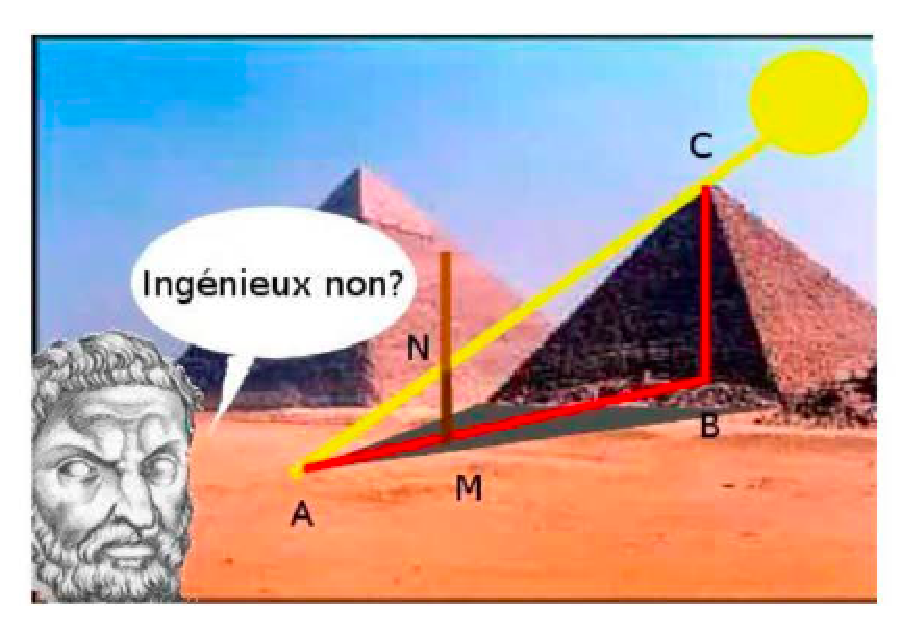
\includegraphics[scale=0.4]{T9}
\end{center}

Les points A, M, B sont alignés, les points A, N, C aussi.

Les droites (MN) et (BC) sont parallèles. On donne:

AM = 5,4 m; MN = 1,39 m et MB = 534,6 m.

Calculer la hauteur BC de la pyramide de Kheops.

Citation de Thalès: "Le rapport que j'entretiens avec mon ombre est le même que celui de la pyramide avec la sienne."
\end{exercice}

\begin{exercice}
On a : OM= 2,8 cm ; ON = 5,4 cm ; OS= 2,7 cm
et OT = 1,4 cm.

\begin{center}
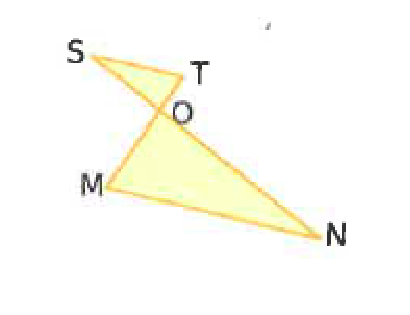
\includegraphics[scale=0.5]{T4}
\end{center}
Démontrer que les droites MN et ST sont parallèles.
\end{exercice}

\begin{exercice}
L'unité de longueur choisie est le mètre. 
\begin{center}
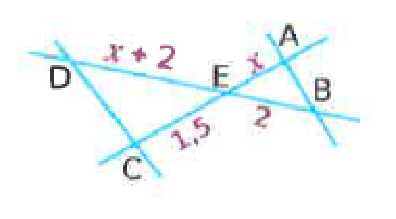
\includegraphics[scale=0.5]{T5}
\end{center}

\begin{enumerate}
\item Pour $x = 2,5$, les droites (AB) et (CD) ne sont pas parallèles. 
Vrai ou faux? Expliquer la démarche.
\item Pour $x = 1$, les droites (AB) et (DC) ne sont pas parallèles. Vrai ou faux ? Expliquer la démarche.
\end{enumerate}
\end{exercice}

\begin{exercice}
ABC est un triangle. D est un point de [AB] et E est un point de (AC) n'appartenant pas à [AC]. On donne AB = 4cm ; AC = 3cm ; AD = 1,2cm et AE = 0,9cm.\\
Alixien a écrit sur sa copie :\\
« Les droites EC et DB sont sécantes en A.\\\\
 D'une part, $\dfrac{AD}{AB}=\dfrac{1,2}{4}=\dfrac{12}{40}=\dfrac{3}{10}$.\\\\
D'autre part, $\dfrac{AE}{AC}=\dfrac{0,9}{3}=\dfrac{9}{30}=\dfrac{3}{10}$.\\\\
Comme $\dfrac{AD}{AB}=\dfrac{AE}{AC}$ alors les droites BC et ED sont parallèles. » 

\begin{enumerate}
\item Quel théorème Alixien a-t-il utilisé ?
\item La réponse d'Alixien est-elle juste ? Sinon, rédiger la bonne réponse..
\end{enumerate}
\end{exercice}

\newpage

%%%%%%%%%%%%%%%%%%%%%%%%%%%%%%%%%%%%%%%%%%%%%%%%%%%

\serie{Divers}

\begin{exercice}
Sur la figure, les droites (EF) et (MP) sont parallèles.
\begin{center}
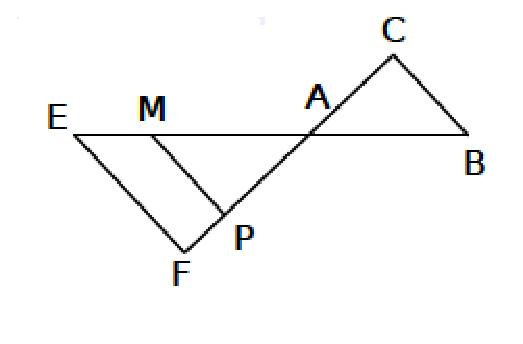
\includegraphics[scale=0.5]{T10}
\end{center}

On sait que AM=6 cm ; MP=4,8cm ; AP=3,6 cm ; EF=6 cm ; AC=4,5 cm et AB=7,5 cm .

\begin{enumerate}
\item Démontrer que le triangle AMP est un triangle rectangle.
\item Calculer AE puis la longueur ME.
\item Démontrer que les droites (MP) et (BC) sont parallèles.
\end{enumerate}
\end{exercice}


\begin{exercice}
Pour consolider un bâtiment, des charpentiers  ont construit un contrefort en bois (les mesures sont en mètre).

\begin{minipage}{0.5\linewidth}
\begin{enumerate}
\item En considérant que le montant [BS] est perpendiculaire au sol, calculer la longueur AS.
\item Calculer les longueurs SM et SN.
\item Démontrer que la traverse [MN] est bien parallèle au sol.
\end{enumerate}

\end{minipage}
\hfill
\begin{minipage}{0.4\linewidth}
\begin{center}
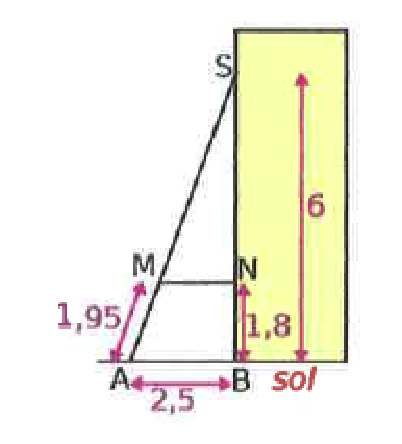
\includegraphics[scale=0.5]{T6}
\end{center}
\end{minipage}
\end{exercice} 











\end{colonne*exercice}




\connaissances


\QCMautoevaluation{Pour chaque question, plusieurs réponses sont
  proposées.  Déterminer celles qui sont correctes.}


\begin{QCM}

\begin{GroupeQCM}

\begin{exercice}Si $RKE$ est rectangle en $K$ alors...
\begin{ChoixQCM}{4}
\item $RK^2 = RE^2 + EK^2$
\item $EK^2 = ER^2 + RK^2$
\item $RE^2 = RK^2 + KE^2$
\item $KE^2 = RE^2 – RK^2$
\end{ChoixQCM}
\begin{corrige}
\reponseQCM{b}
\end{corrige}
\end{exercice}

\begin{exercice}$ABC$ est rectangle en $A$ ; $AB = 5$ et $BC = 7$ (en cm). L'arrondi au dixième de $AC$ est...
\begin{ChoixQCM}{4}
\item 8,6 cm
\item 4,8 cm
\item 4,89 cm
\item 4,9 cm
\end{ChoixQCM}
\begin{corrige}
\reponseQCM{d}
\end{corrige}
\end{exercice}

\begin{exercice}Si $KG^2 \neq KC^2 + CG^2$ alors...
\begin{ChoixQCM}{4}
\item $KCG$ n'est pas rectangle
\item $KCG$ peut être rectangle
\item $KCG$ n'est pas rectangle en $C$
\item $KCG$ est quelconque
\end{ChoixQCM}
\begin{corrige}
\reponseQCM{b c}
\end{corrige}
\end{exercice}

\begin{exercice}Si $M\in [AC]$, $N\in [BC]$ et $(MN)//(AB)$ alors...

\definecolor{zzttqq}{rgb}{0.6,0.2,0.}
\begin{tikzpicture}[scale=0.75][line cap=round,line join=round,>=triangle 45,x=1.0cm,y=1.0cm]
\clip(1.16,0.4) rectangle (5.8,3.56);
\fill[color=zzttqq,fill=zzttqq,fill opacity=0.1] (2.,1.) -- (5.,1.) -- (5.,3.) -- cycle;
\draw [color=zzttqq] (2.,1.)-- (5.,1.);
\draw [color=zzttqq] (5.,1.)-- (5.,3.);
\draw [color=zzttqq] (5.,3.)-- (2.,1.);
\draw (4.,1.)-- (3.98461538462,2.32307692308);
\begin{scriptsize}
\draw [color=black] (2.,1.)-- ++(-1.5pt,-1.5pt) -- ++(3.0pt,3.0pt) ++(-3.0pt,0) -- ++(3.0pt,-3.0pt);
\draw[color=black] (1.66,1.14) node {$C$};
\draw [color=black] (5.,1.)-- ++(-1.5pt,-1.5pt) -- ++(3.0pt,3.0pt) ++(-3.0pt,0) -- ++(3.0pt,-3.0pt);
\draw[color=black] (5.26,1.02) node {$B$};
\draw [color=black] (5.,3.)-- ++(-1.5pt,-1.5pt) -- ++(3.0pt,3.0pt) ++(-3.0pt,0) -- ++(3.0pt,-3.0pt);
\draw[color=black] (5.14,3.28) node {$A$};
\draw [color=black] (4.,1.)-- ++(-1.5pt,-1.5pt) -- ++(3.0pt,3.0pt) ++(-3.0pt,0) -- ++(3.0pt,-3.0pt);
\draw[color=black] (4.,0.8) node {$N$};
\draw [color=black] (3.98461538462,2.32307692308)-- ++(-1.5pt,-1.5pt) -- ++(3.0pt,3.0pt) ++(-3.0pt,0) -- ++(3.0pt,-3.0pt);
\draw[color=black] (3.92,2.78) node {$M$};
\end{scriptsize}
\end{tikzpicture}
\begin{ChoixQCM}{4}
\item $\dfrac{AM}{AC}=\dfrac{BN}{BC}=\dfrac{MN}{AB}$
\item $\dfrac{CM}{CN}=\dfrac{CA}{CB}=\dfrac{MN}{AB}$
\item $\dfrac{CM}{CA}=\dfrac{CN}{CB}=\dfrac{MN}{AB}$
\item $\dfrac{CM}{CA}=\dfrac{CB}{CN}=\dfrac{MN}{AB}$
\end{ChoixQCM}
\begin{corrige}
\reponseQCM{c}
\end{corrige}
\end{exercice}

\begin{exercice}Dans le cas précédent,  $CM = 4,5$ ; $MA = 3$ et $CN = 3$ donc...
\begin{ChoixQCM}{4}
\item $CB = 2$
\item $CB = 5$
\item $BN = 2$
\item $CB = \dfrac{9}{5}$
\end{ChoixQCM}
\begin{corrige}
\reponseQCM{b}
\end{corrige}
\end{exercice}


\begin{exercice}

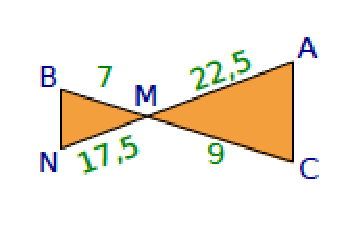
\includegraphics[scale=0.5]{T11}
\begin{ChoixQCM}{4}
\item $(AC)$ et $(BN)$ sont parallèles
\item $(AC)$ et $(BN)$ ne sont pas parallèles
\item On ne peut pas savoir si $(AC)$ 
et $(BN)$ sont parallèles
\item $\dfrac{NB}{AC}=\dfrac{MB}{MC}$
\end{ChoixQCM}
\begin{corrige}
\reponseQCM{a d}
\end{corrige}
\end{exercice}


\end{GroupeQCM}
\end{QCM}

  




\pagebreak





%\themaC
%\chapter{Equations et inéquations de degré 1}\label{ChDegre1}

\begin{acquis}
\begin{itemize}
\item Savoir résoudre des équations (Rappel) et des inéquations du 1er degré;
\item Savoir écrire des inégalités sous forme d'Intervalles réels;
\item Savoir mettre en équation ou en inéquation un problème.
\end{itemize}
\end{acquis}
\exercicesbase
\begin{colonne*exercice}

\serie{Equations}

\begin{exercice}
\begin{enumerate}
\item Le nombre 2 est-il solution de l'équation\\
 $5x+1=2x+7$?
\item Le nombre $\dfrac{1}{2}$ est-il solution de l'équation\\ $3x-8=5x-11$?
\end{enumerate}
\end{exercice}


\begin{exercice}
Résoudre les équations suivantes:

\renewcommand{\arraystretch}{0.8}
\begin{tabular}{p{4cm}p{4cm}}
(a) $5x=3x+3$ & (b) $8x=12x+4$\\
&\\
(c) $4-7y=10y$ & (d) $7x+1=4-x$\\
&\\
(e) $2+3x=7+3x$ & (f) $-x=-8x-3,4$\\
&\\
(g) $5x+1=5x-1$ & (h) $5x=0$\\
\end{tabular}
\end{exercice}

\begin{exercice}
Résoudre les équations suivantes:

\renewcommand{\arraystretch}{0.8}
\begin{tabular}{p{6cm}p{1cm}}
(a) $7x-(5x+3)=5(x-3)+2$\\
&\\
(b) $4y+3(4y-2)=3(y+1)$\\
&\\
(c) $\dfrac{x}{5}-\dfrac{3x-2}{15}=\dfrac{1-x}{3}$\\
&\\
(d) $-4=\dfrac{-4x+30}{5}$\\
&\\
(e) $\dfrac{2x}{7}+\dfrac{3}{14}=\dfrac{x}{7}-\dfrac{1}{14}$\\
&\\
(f) $\dfrac{2}{5}x-\dfrac{1}{9}=\dfrac{3}{9}x+\dfrac{4}{5}$\\
\end{tabular}
\end{exercice}

\serie{Equations et problèmes}

\begin{exercice}
En multipliant un nombre par 12, on l’augmente de 253.\\
Quel est ce nombre?
\end{exercice}

\begin{exercice}
Le quadruple d’un nombre, diminué de 7, est égal au double de ce nombre, augmenté de 19.\\
Quel est ce nombre?
\end{exercice}


\begin{exercice}
Une personne a dépensé le tiers de son argent, puis le cinquième de l’argent restant et il lui reste encore 14 CHF.\\
Combien d’argent avait-elle initialement ?
\end{exercice}

\begin{exercice}
Combien y a-t-il d'élèves dans une classe sachant que le tiers travaille, deux cinquièmes bavardent et les huit qui restent somnolent?
\end{exercice}


\begin{exercice}
Le ciné-club d'une ville propose deux tarifs :
\begin{description}
\item Tarif A : une carte d'adhésion pour l'année coûtant 63 CHF, puis 4,5 CHF par séance;
\item Tarif B : 15 CHF par séance sans carte d'adhésion.
\end{description}

\begin{enumerate}
\item Calculer, pour chaque tarif, le prix payé pour 8 séances.
\item On appelle $x$ le nombre de séances. Exprimer en fonction de $x$ le prix payé avec le tarif A, puis avec le tarif B.
\item Quel est le nombre de séances pour lequel le tarif A est égal au tarif B ?
\end{enumerate}
\end{exercice}

\begin{exercice}
Quentin pense à un nombre, lui ajoute 11, multiplie le tout par 3 et au résultat obtenu il retranche 3. Joey obtient 51. Quel est le nombre de départ ?
\end{exercice}

\serie{Intervalles}

\begin{exercice}
Ecrire sous forme d’intervalle les inégalités ci-dessous et dessiner ces intervalles sur la droite réelle.\\

\renewcommand{\arraystretch}{0.8}
\begin{tabular}{p{4cm}p{4cm}}
(a) $-5\leq x \leq 2$ & (b) $-2 < x < 4$\\
&\\
(c) $0<x<7$ & (d) $-6 \leq x < 0$\\
&\\
(e) $x<-2$ & (f) $1<x$\\
&\\
(g) $x<0$ ou $4<x<10$ & (h) $x<3$ ou $x\geq 4$\\
&\\
(i) $x<5$ et $x\geq 4$ & (j) $x\geq -3$ et $x< 4$\\
\end{tabular}
\end{exercice}

\begin{exercice}
Ecrire sous forme d’inégalités et d’intervalles chacun des dessins ci-dessous.\\

\renewcommand{\arraystretch}{0.8}
\begin{tabular}{p{6cm}p{1cm}}
(a) 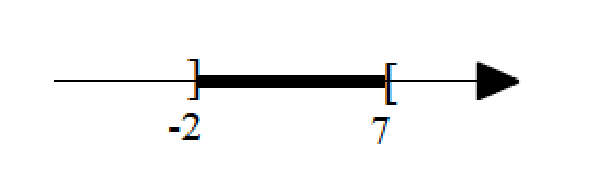
\includegraphics[scale=0.5]{I1}
 &\\
 (b) 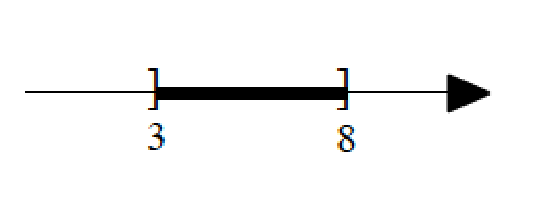
\includegraphics[scale=0.5]{I2}
&\\
(c) 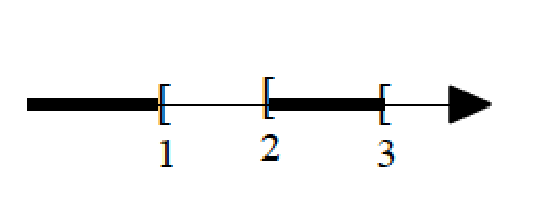
\includegraphics[scale=0.5]{I3}
\end{tabular}
\end{exercice}

\serie{Inéquations}

\begin{exercice}
Résoudre les inéquations suivantes:\\

\renewcommand{\arraystretch}{0.8}
\begin{tabular}{p{4cm}p{4cm}}
(a) $7x-8 > 6$ & (b) $4x+9>-21$\\
&\\
(c) $4-9x<7$ & (d) $2-6x\geq26$\\
&\\
(e) $2+7x>16$ & (f) $12>3-3x$\\
\end{tabular}
\end{exercice}

\begin{exercice}
Résoudre les inéquations suivantes:\\

\renewcommand{\arraystretch}{0.8}
\begin{tabular}{p{4cm}p{4cm}}
(a) $5x-7 > 11x+9$ & (b) $5x+5<5x$\\
&\\
(c) $2(4x-1)\leq 3x-6$ & (d) $2x-4 \geq 7-8x$\\
&\\
(e) $2-5x\geq 3(x-9)$ & (f) $\dfrac{1}{2}x-5>\dfrac{1}{4}x+3$\\
\end{tabular}
\end{exercice}

\begin{exercice}
Résoudre les inéquations suivantes:\\

\renewcommand{\arraystretch}{0.8}
\begin{tabular}{p{6cm}p{1cm}}
(a) $3(x+1)-x\leq1+2(1+x)$\\
&\\
(b) $-\dfrac{3}{5}x-6 < - \dfrac{2}{5}x+7$\\
&\\
(c) $-3(2-7x)+8-(3-3x)\geq 7-(3+5x)$\\
&\\
(d) $\dfrac{1}{5}-\dfrac{4}{3}\geq2\left( 1-\dfrac{5}{6}x\right) $\\

\end{tabular}
\end{exercice}

\begin{exercice}
Résoudre les inéquations suivantes:\\

\renewcommand{\arraystretch}{0.8}
\begin{tabular}{p{6cm}p{1cm}}
(a) $2x-(3x+4)\geq8x-7$\\
&\\
(b) $4+3(4x-5)\leq5-(7-2x)$\\
&\\
(c) $9-(3+7x)<2x+3(x-4)$\\
&\\
(d) $2x-\dfrac{2}{3}<2-\dfrac{x+1}{3}$\\

\end{tabular}
\end{exercice}

\begin{exercice}
\begin{enumerate}
\item Résoudre l'inéquation: $2x-7(3x-2)\leq 34 - 9 x$ et représenter graphiquement les solutions.
\item Résoudre l'inéquation: $6(3x-5) < 9-3(1-2x)$ et représenter graphiquement les solutions.
\item En utilisant les résultats précédents, représenter graphiquement les valeurs de $x$ qui vérifient: $2x-7(3x-2)\leq 34 - 9 x$ et $6(3x-5) < 9-3(1-2x)$.
\end{enumerate}
\end{exercice}

\serie{Inéquations et problèmes}

\begin{exercice}
La société Allo propose un abonnement téléphonique de 98 CHF par mois et1,30 CHF par minute de communication. 

La société Lalo propose un abonnement téléphonique de 95 CHF par mois et 1,45 CHF  par minute de communication.

On désigne par $x$  le nombre de minutes de communication par mois.

\begin{enumerate}
\item Exprimer en fonction de x  le montant d’une facture de Allo, puis le montant d’une facture de Lalo.
\item Pour quelles durées de communications mensuelles a-t-on intérêt à choisir Allo ?
\end{enumerate}
\end{exercice}

\begin{exercice}
Une entreprise de recherche emploie 27 informaticiens et 15 mathématiciens. 

On envisage d’embaucher le même nombre $x$  d’informaticiens et de mathématiciens.

Combien faut-il embaucher de spécialistes de chaque sorte pour que le nombre de mathématiciens soit au moins égal aux deux tiers du nombre d’informaticiens ?
\end{exercice}

\begin{exercice}
La longueur d’un rectangle dépasse de 7 dm sa largeur. 

On sait que son périmètre est compris entre 20 dm et 26 dm. 

Que peut-on dire au sujet de sa largeur ? 
\end{exercice}

\begin{exercice}
Paul a 32 ans et Mafalda a 5 ans. 

Pendant combien d’années l’âge de Paul restera-t-il plus grand que quatre fois celui de Mafalda ?  
\end{exercice}
\end{colonne*exercice}


\connaissances

\QCMautoevaluation{Pour chaque question, plusieurs réponses sont
  proposées.  Déterminer celles qui sont correctes.}

\begin{QCM}
  \begin{GroupeQCM} 
  
    \begin{exercice}
      L'équation $2x – 6 = 2(– 2 + x)$...
      \begin{ChoixQCM}{4}
      \item admet 0 pour solution
      \item admet 2 pour solution
      \item a les mêmes solutions que $0x = 2$
      \item n'a pas de solution
      \end{ChoixQCM}
\begin{corrige}
     \reponseQCM{cd}
   \end{corrige}
    \end{exercice}
    
      \begin{exercice}
      « Le double de la somme d'un nombre et de 3 est égal à la moitié de ce nombre, augmentée de 5 »
      \begin{ChoixQCM}{4}
      \item $\dfrac{x}{2} + 3 = 2x + 5$
      \item $2x + 3 = \dfrac{x}{2} + 5$
      \item $2(x + 3) = \dfrac{x+5}{2}$
      \item ce nombre n'a pas d'écriture décimale
      \end{ChoixQCM}
\begin{corrige}
     \reponseQCM{b}
   \end{corrige}
    \end{exercice}
    
      \begin{exercice}
     $4x + 3 < 9$ donc...
   \begin{ChoixQCM}{4}
      \item $4x > 9 – 3$
      \item $\dfrac{4x+3}{9}< 1$
      \item $x$ peut être égal à 10
      \item $x < 1,5$
      \end{ChoixQCM}
\begin{corrige}
     \reponseQCM{bd} % ici deux réponses justes
   \end{corrige}
    \end{exercice}
    
      \begin{exercice}
     L'ensemble des nombres strictement supérieurs à 3 est représenté par...
      \begin{ChoixQCM}{4}
      \item 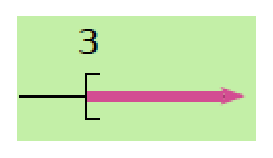
\includegraphics[scale=0.5]{I4}
      \item 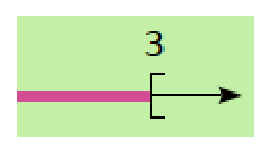
\includegraphics[scale=0.5]{I5}
      \item \includegraphics[scale=0.5]{I6}
      \item 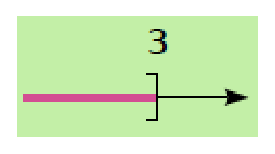
\includegraphics[scale=0.5]{I7}
      \end{ChoixQCM}
\begin{corrige}
     \reponseQCM{c}
   \end{corrige}
    \end{exercice}
    
      \begin{exercice}
    L'inéquation qui a pour solutions tous les nombres  inférieurs ou égaux à $− 2$  est...
      \begin{ChoixQCM}{4}
      \item $3x < − 6$
      \item $x+2\geq 4x+8$
      \item $-5x\leq 10$
      \item $8\geq x+10$
      \end{ChoixQCM}
\begin{corrige}
     \reponseQCM{bd} % ici deux réponses justes
   \end{corrige}
    \end{exercice}
    
      \begin{exercice}
      L'inéquation $2x + 5 \leq 2x + 6$...
      \begin{ChoixQCM}{4}
      \item admet tout nombre positif comme solution
      \item a une infinité de solutions
      \item admet 7 comme solution
      \item n'a pas de solution
      \end{ChoixQCM}
\begin{corrige}
     \reponseQCM{abc} 
   \end{corrige}
    \end{exercice}
   


\end{GroupeQCM}
\end{QCM}

  



\pagebreak






%\themaG
%\include{Quadrilateres/Quadrilateres}

%\themaC
%\include{NbsRelatifs/NbsRelatifs}

%\themaG
%\include{PerimetresAires/PerimetresAires}

%\AfficheListeMethodes
\AfficheCorriges[2]
%\AfficheLexique

\end{document}

%%% Local Variables: 
%%% mode: latex
%%% TeX-master: t
%%% End: 
